\documentclass{beamer}

%% \documentclass[handout]{beamer}
%% % use this with the [handout] option to create handouts for the audience
%% \usepackage{pgfpages}
%% \pgfpagesuselayout{2 on 1}[a4paper,border shrink=5mm]

\mode<presentation>
{
  \usetheme{Diku}
% set this to your preferences:
  \setbeamercovered{invisible}
%  \setbeamercovered{transparent}
}

\usepackage{graphicx}
\usepackage{epic}

\usepackage{amsmath}
\usepackage{amssymb}
\usepackage{amsthm}

\newcommand{\basetop}[1]{\vtop{\vskip-1ex\hbox{#1}}}
\newcommand{\source}[1]{\let\thefootnote\relax\footnotetext{\scriptsize\textcolor{kugray1}{Source: #1}}}

% for coloured code citation in text:
\usepackage{fancyvrb}

%%%%%%%%%%%%%%%%%%%%%%%%%%%%%%%%%
%%%%%    code sections   %%%%%%%%
%%%%%%%%%%%%%%%%%%%%%%%%%%%%%%%%%

% code highlighting commands in own block
\DefineVerbatimEnvironment{code}{Verbatim}{fontsize=\scriptsize}
\DefineVerbatimEnvironment{icode}{Verbatim}{fontsize=\scriptsize}

% Fancy code with color commands:
\DefineVerbatimEnvironment{colorcode}%
        {Verbatim}{fontsize=\scriptsize,commandchars=\\\{\}}

%%%%%%%%%%%%%%%%%%%%%%%%%%%%%%%%%%
%%%%%    some coloring    %%%%%%%%

\definecolor{Red}{RGB}{220,50,10}
\definecolor{Blue}{RGB}{0,51,102}
\definecolor{Yellow}{RGB}{102,51,0}
\definecolor{Orange}{RGB}{178,36,36}
\definecolor{Grey}{RGB}{180,180,180}
\definecolor{Green}{RGB}{20,120,20}
\definecolor{Purple}{RGB}{160,50,100}
\newcommand{\red}[1]{\textcolor{Red}{{#1}}}
\newcommand{\blue}[1]{\textcolor{Blue}{{#1}}}
\newcommand{\yellow}[1]{\textcolor{Yellow}{{#1}}}
\newcommand{\orange}[1]{\textcolor{Orange}{{#1}}}
\newcommand{\grey}[1]{\textcolor{Grey}{{#1}}}
\newcommand{\green}[1]{\textcolor{Green}{{#1}}}
\newcommand{\purple}[1]{\textcolor{Purple}{{#1}}}




% use "DIKU green" from our color theme for \emph
\renewcommand{\emph}[1]{\textcolor{structure}{#1}}
% use some not-too-bright red for an \emp command
\definecolor{DikuRed}{RGB}{130,50,32}
\newcommand{\emp}[1]{\textcolor{DikuRed}{ #1}}
\definecolor{CosGreen}{RGB}{10,100,70}
\newcommand{\emphh}[1]{\textcolor{CosGreen}{ #1}}
\definecolor{CosBlue}{RGB}{55,111,122}
\newcommand{\emphb}[1]{\textcolor{CosBlue}{ #1}}
\definecolor{CosRed}{RGB}{253,1,1}
\newcommand{\empr}[1]{\textcolor{CosRed}{ #1}}

\newcommand{\mymath}[1]{$ #1 $}
\newcommand{\myindx}[1]{_{#1}}
\newcommand{\myindu}[1]{^{#1}}

\newcommand{\Fasto}{\textsc{Fasto}\xspace}


%%%%%%%%%%%%%%%%%%%%

\title[Processor]{Mostly-Static Processor Architecture}

\author[C.~Oancea]{Cosmin E. Oancea\\{\tt cosmin.oancea@diku.dk}}

\institute{Department of Computer Science (DIKU)\\University of Copenhagen}


\date[Sept 2014]{September 2014 Compiler Lecture Notes}


\begin{document}

\titleslide

\begin{frame}
\frametitle{Structure of a Compiler}

\begin{tabular}{ccc}
Program text&&\\
$\downarrow$ &&\\
\framebox{Lexical analysis} && Binary machine code\\
$\downarrow$ && $\uparrow$ \\
Symbol sequence && \textcolor{gray}{\framebox{Assembly and linking}} \\
$\downarrow$ && $\uparrow$ \\
\framebox{Syntax analysis} && Ditto with named registers\\
$\downarrow$ && $\uparrow$ \\
Syntax tree && \framebox{Register allocation} \\
$\downarrow$ && $\uparrow$ \\
\framebox{Typecheck} && Symbolic machine code\\
$\downarrow$ &&  $\uparrow$ \\
Syntax tree  && \framebox{Machine code generation} \\
$\downarrow$ && $\uparrow$ \\
\framebox{Intermediate code generation} &$\longrightarrow$ & Interm code + \red{Optimizations}
\end{tabular}

\end{frame}



%%%%%%%%%%%%%%%%%%%%%%%%%%%%%%%%%%%%%%%%%%%%%%%%%%%%%%%%%%%%%%%%%%%%%%
%%%%%%%%%%%%%%%%%%%%%%%%%%%%%%%%%%%%%%%%%%%%%%%%%%%%%%%%%%%%%%%%%%%%%%
%%%%%%%%%%%%%%%%%%%%%%%%%%%%%%%%%%%%%%%%%%%%%%%%%%%%%%%%%%%%%%%%%%%%%%


\begin{frame}[fragile,t]
\frametitle{Overview}

\begin{itemize}
    \item Processor (\& ISA): ``the brain'', drive the architectural design.\smallskip
 
    \item Will recall MIPS and exceptions, which, albeit implemented in software, 
            impose architectural constraints.\smallskip
    \item Starting Point: 5-stage pipeline, executing instructions in 
            program order. At this level we look at how to best exploit ILP.\smallskip
    \item Mechanisms to handle hazards: forwarding, stalling, flushing.\smallskip
    \item Look at 5-stage static pipeline extensions:
        \begin{itemize}
            \item superpipelined: deeper pipelines, clocked faster, supporting
                    more complex instructions, e.g., floating point,
            \item superscalar: fetch and execute multiple instrs in each cycle,
            \item core multi-threading: as a simple solution to resolving hazards.\smallskip
        \end  {itemize}
\end  {itemize}

\end{frame}

\begin{frame}[fragile,t]
\frametitle{Overview Continuation}

\begin{itemize}
    \item Dynamically Scheduled OoO Processors are NOT covered until the end of the course!
        \begin{itemize}
            \item daunting task because instructions are
                    executed out of order, but data dependencies, conditional branches outcome,
                    and exceptions must be correctly processed (as if in program order).
            \item requires complex hardware support for speculative execution.
        \end  {itemize}\bigskip

    \item Complexity of OoO Processors prevents wide-superscalar
            pipelines $\Rightarrow$ next lectures on software track study
            compiler optimizations to keep hwd simple \& clock rates high:
        \begin{itemize}
            \item VLIW: simple hardware allowing a large number of instrs to be     
                        processed every cycle: data dependencies, speculative execution 
                        and exceptions are handled statically. 
            \item Vector Processors: compiler restructures code into vector instructions,
                    in which the same instruction is applied on many scalar operands.
                    Can be deeply pipelined at high-clock rates. 
        \end  {itemize}\bigskip
\end  {itemize}

\end{frame}

\section{Instruction Set Architectures (ISA)}

\begin{frame}[fragile]
	\tableofcontents[currentsection]
\end{frame}


\subsection{RISC vs CISC}
\begin{frame}[fragile,t]
\frametitle{ISA: RISC vs CISC}

{\bf Reduced Instruction Set Architecture (RISC):}
\begin{itemize} 
    \item start with the minimum \# of primitive instrs \& add only 
            if justified by performance gains.\smallskip
    \item Constant instr size, regular formats $\Rightarrow$ simplified decoding, 
            promotes pipelining \& short cycle time.
\end  {itemize}

\bigskip

{\bf Complex Instruction Set Architecture (CISC):}
\begin{itemize} 
    \item Premises: compact instr stream $\Rightarrow$ effective time/space 
            instr-memory utilization $\Rightarrow$ variable instr length and format.\smallskip
    \item Misguided tendency to provide complex ISA to help assembly programmers or to 
            compile high-level languages.\smallskip
    \item DEC Vax-11 ISA successful in the 70-80s.\\
          Intel iAPX432 1980s zenith of complexity: $>$200 opcodes, 6-300 bits instr length   
            with Huffman coding, in the context of ADA.
\end  {itemize}
\end{frame}

\begin{frame}[fragile,t]
\frametitle{ISA: RISC vs CISC (Continuation)}

\begin{block}{Execution of a CISC instruction}
\begin{columns}
\column{0.33\textwidth}
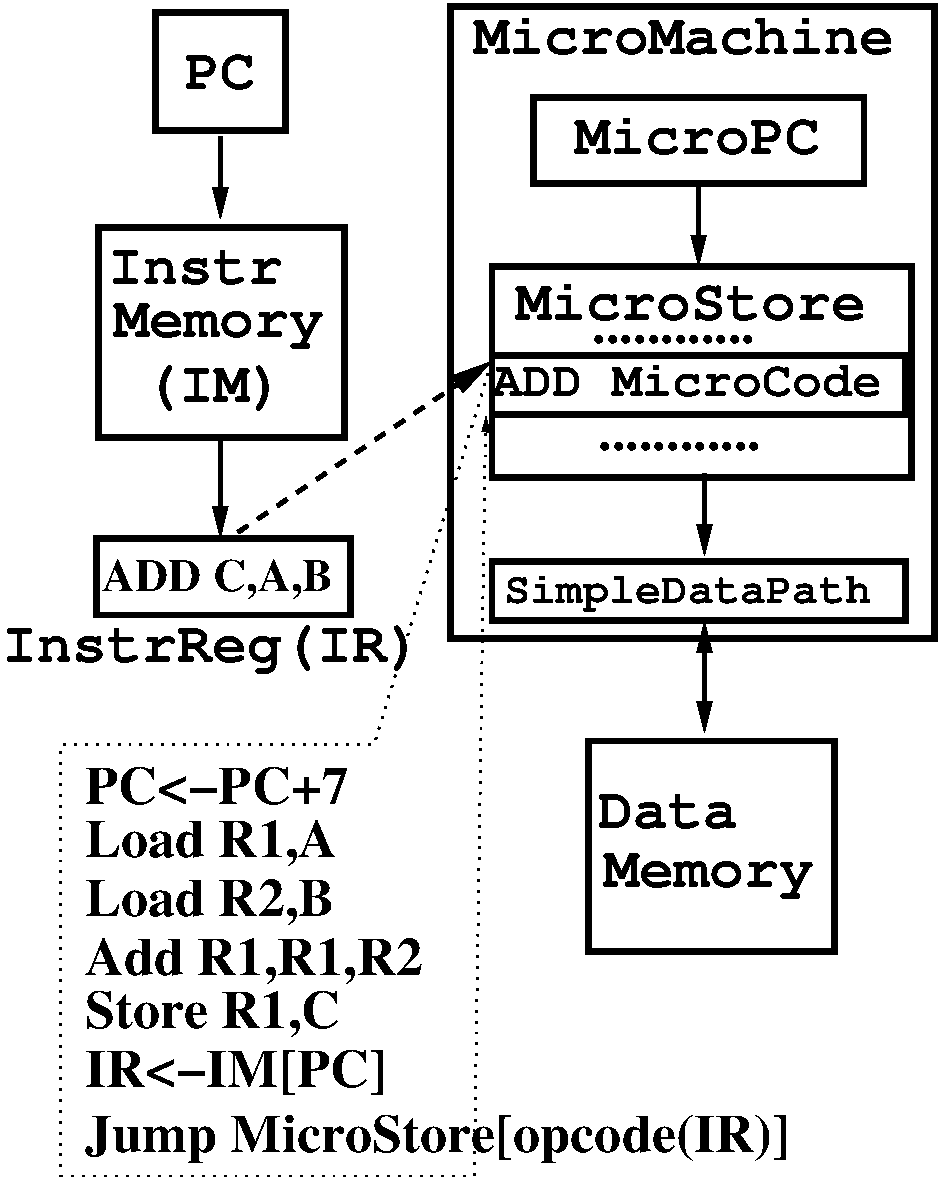
\includegraphics[width=20ex]{Figures/CISCarch}
\column{0.62\textwidth}
\begin{scriptsize}
Complex instr fetched from {\tt InstrMemory} \& decoded:
\begin{itemize}
    \item opcode and operand types determines the entry in {\tt Microstore}
            where its sequence of $\mu$instrs reside,
    \item $\mu$instructions are similar to the one of MIPS,
    \item the last $\mu$instruction execution directs the {\tt InstrMemory}
            to fetch the next complex instr. 
    \item Inefficient execution because $\mu$program exhibit little ILP \&
            extra cycles are required for the interpretation of ANY
            instr (simple or complex).   
    \item RISC: removes the interpretation overhead by compiling directly to 
            $\mu$code, which is exposed to compiler optimizations.
\end  {itemize}  
\end{scriptsize}
\end{columns}
\end{block}

\begin{scriptsize}
\begin{itemize}
\item RISC \& CISC refers NOT to hwd simplicity (cost of implementing CISC is marginal).
      Today architectures are CISC due to legacy concerns, but morally RISC:
\item CISC instr translated to a sequence of RISC, executed by
            a RISC-ISA mechanism.
\item CISC: IBM System370..., IntelX86 (Pentium4,AMD Turion), Motorola 68000,
\item RISC: SunSPARC(SPARCT2), PowerPC(601 IBM), Alpha(DEC), IA64(Itanium2).  
\end  {itemize}
\end{scriptsize}
\end{frame}

\subsection{MIPS Instruction Format \& Mixes}

\begin{frame}[fragile,t]
\frametitle{MIPS Instruction Set}

Instructions in 32-bit format aligned in memory. Addresses assumed aligned (why?).
%
Each instr has one {\tt opcode} and up to three operands:\smallskip
\begin{scriptsize}
\begin{description}
\item[Arithmetic/Logic:] use integer registers {\tt R0$\ldots$R31}.
                         Unsigned ({\tt ADDU,SUBU,MULTU}) and logical ({\tt OR,AND,NOR,NAND}) 
                         instructions do not raise exceptions.\\
                         Signed instr ({\tt ADD,SUB,MULT}) raise under/overflow exceptions.\\
                         {\tt ADD R1,R2,R3 $\equiv$ R1$\leftarrow$R2+R3} and
                         {\tt ADDI R1,R2,\#8 $\equiv$ R1$\leftarrow$R2+8}.\\
                         {\tt SLT R1,R2,R3 $\equiv$ R1 $\leftarrow$ if R2 < R3 then 1 else 0}.\smallskip
\item[Floating Point:]   Numbers in sign-exponent-mantisa widens the range of representable numbers.
                         Use float registers {\tt F0$\ldots$F31}. Can be executed as procedures/macros,
                         but much faster in hardware. No immediate field!\\
                         Single ({\tt ADD.S,SUB.S,MUL.S}) and double ({\tt ADD.D$\ldots$})
                         precision instrs.\\ 
                         \emp{A double register is hold in 2 consecutive registers and is even numbered:}\\
                         {\tt MUL.S F1,F2,F3 $\equiv$ F1$\leftarrow$F2*F3} and
                         {\tt ADD.D F0,F2,F4 $\equiv$ F0$\leftarrow$F2+F4}.\smallskip
\item[Memory Access:] move operands from/to memory: 1 value reg \& 1 address reg \& 1 displ.\\
                      {\tt LB,LH,LW,LD,L.S,L.D} loads a byte, half/single/double integer word,
                        and a single/double float. Similar for store {\tt SB,SH,SW,SD,S.S,S.D}:\\
                        {\tt LW R1,8(R2) $\equiv$ R1$\leftarrow$MEM[R2+8]} and
                        {\tt SW R1,8(R2) $\equiv$ MEM[R2+8]$\leftarrow$R1}.\smallskip
\item[Branch/Jump:]   %{\em Branches} use PC-relative targets, 
                      {\tt BNE R1,R2,loop} branches when {\tt R1$\neq$R2}; branches 
                        use {\tt PC}-relative targets\\ 
                        {\tt SLT R1,R2,R3; BEZ R1,loop $\equiv$ if R2 $\geq$ R3 then goto loop}.\\
                      Jump to an immediate-field ({\tt J target}) or to a register target 
                        ({\tt JR R1}) sets {\tt PC} to target's value.  
                      Jump-And-Link ({\tt JAL target}), used for procedure calls,
                        first saves the return address in {\tt R31} then jumps.
\end  {description}
\end{scriptsize}
\end{frame}


\begin{frame}[fragile,t]
\frametitle{Instruction Formats}

Most instructions may be executed in one cycle; complex ones require more cycles,
e.g, integer/float multiplication/division.\smallskip

Operand addresses must be aligned (address is a multiple of its size)
$\Rightarrow$ simplifies mem interface (operand cannot span two cache lines).

\bigskip

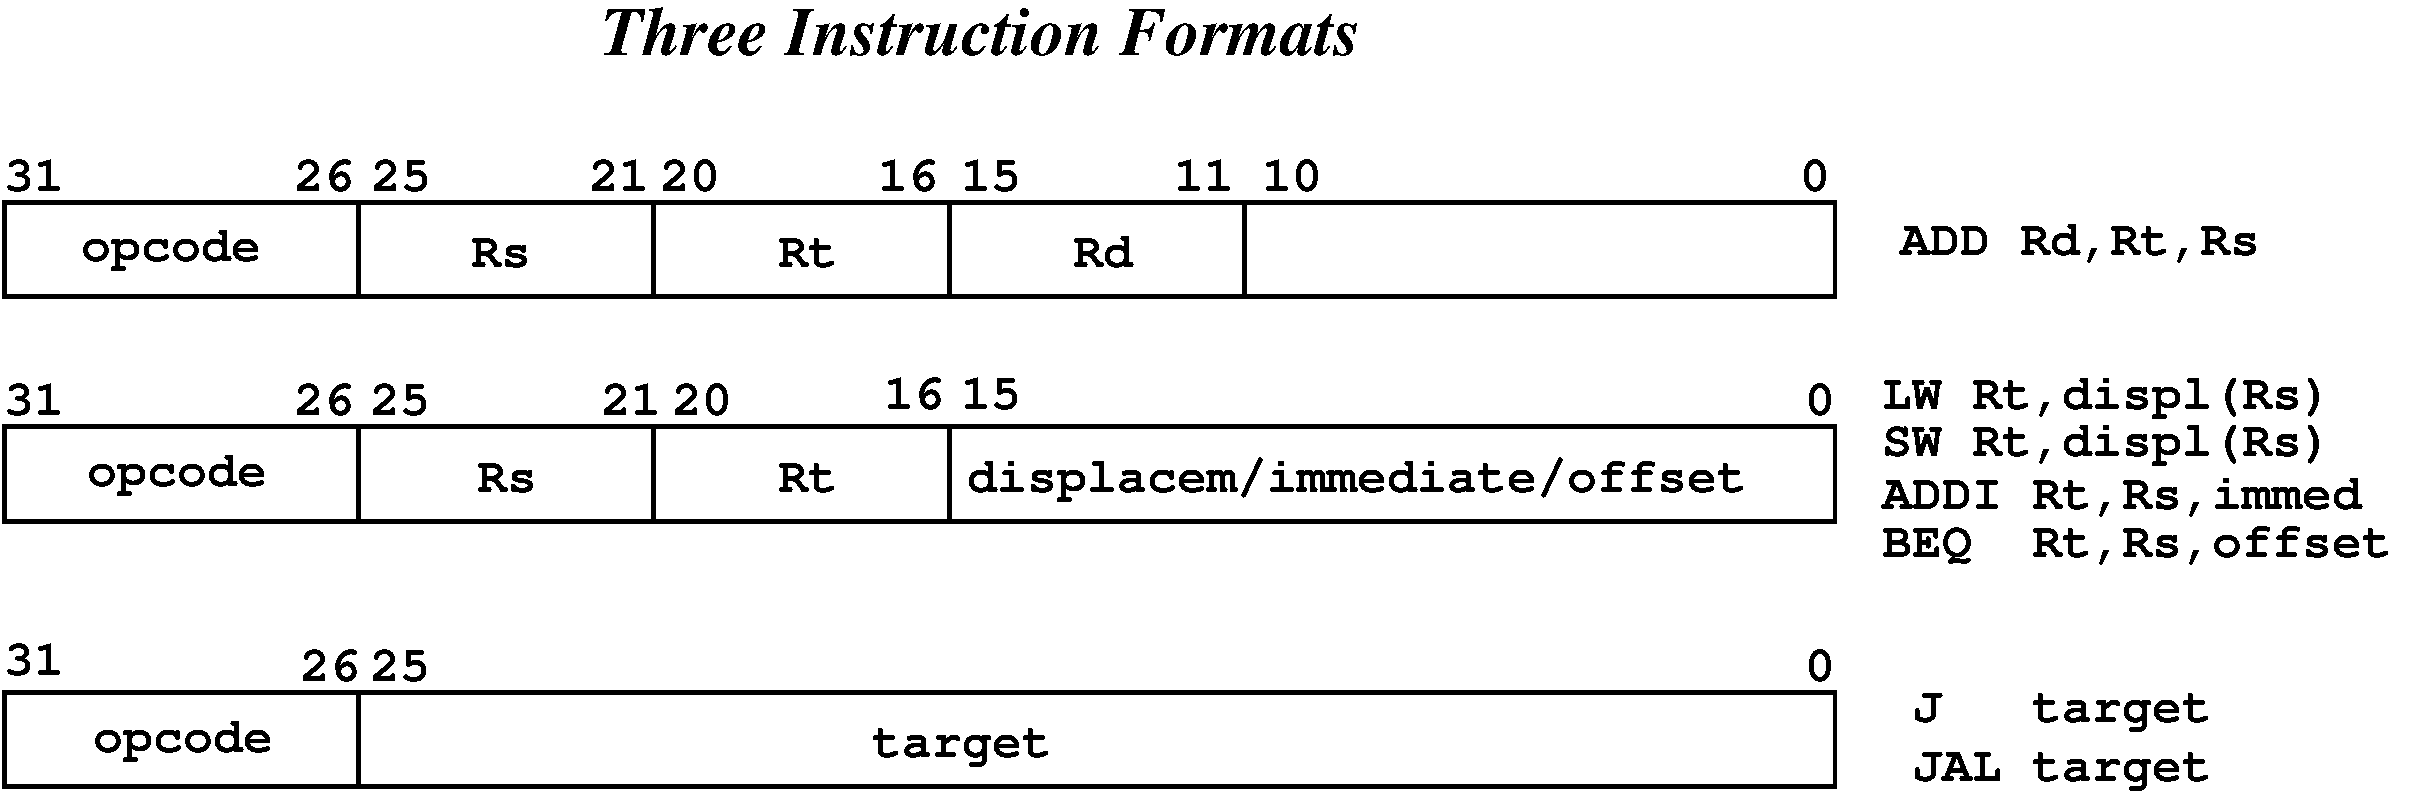
\includegraphics[width=70ex]{Figures/InstrFormats}

\end{frame}

\begin{frame}[fragile,t]
\frametitle{Instruction Mixes}

\begin{scriptsize}
\begin{description}
\item[Static Mixes:] the distribution of instruction types in a program, e.g.,
                        used to determine the size of instruction caches.
\item[Dynamic Mix:] refers to the number of executed instructions, e.g.,
                        instructions in a loop are repeatedly executed.
                    \emp{Used as a primary guideline in processor design.}
\item[Table Below] shows a rough estimate of the dynamic mix 
                    of integer benchmarks:
\end{description}
\end{scriptsize}

\bigskip

\begin{scriptsize}
\begin{tabular}{lrl}
\hline
OpCode Class & Fraction & CPI  \\\hline
Load         & 25\%     & \alert{high} \\
Store        & 12\%     & low  \\
ALU          & 40\%     & low  \\
Branches     & 20\%     & \alert{high} \\
Jump         & 2\%      & low  \\
JAL          & 1\%      & low  \\
\end{tabular}
\end{scriptsize}

\bigskip

\begin{scriptsize}
\begin{description}
\item[Loads] high CPI is due to the memory/bandwidth wall.
\item[Branches] high CPI is because they break the predictability 
                of the segment of instructions fetched in the pipeline.
\item[Processor Design] must address these and other issues.
\end{description}
\end{scriptsize}
\end{frame}

\subsection{Exceptions}

%, Traps, Interrupts
\begin{frame}[fragile,t]
\frametitle{Exceptions}

%\begin{scriptsize}
\begin{itemize}
\item \emp{Rare events} triggered by hardware \& direct the processor
            to execute a handler.\smallskip

\item Similar with branches (share same hardware), but the difference is that 
            the  exception handler is NOT explicitly scheduled in code.\smallskip

\item Exception handling is part of ISA specification:
    \begin{description}
        \item[Imprecise] e.g., hwd failure, mem-access violations, are
                NOT synchronized with an instruction because process is terminated
                after handler.    

        \item[Precise] e.g., under/overflow, page faults @ instruction {\tt i}.\\
            Instrs preceding {\tt i} must finish \& instrs {\tt i} and following
            aborted. Execution resumed from instr {\tt i}.
    \end  {description}\smallskip

\item \emp{Precise exceptions} place constraints on hardware \& compiler:
    \begin{itemize}
        \item exceptions are rare and unpredictable $\Rightarrow$
        \item no need to speed up the handling BUT build the mechanism \& minimize 
                its common-case (conservative) overhead.
    \end  {itemize}
\end{itemize}
%\end{scriptsize}


\end{frame}


\begin{frame}[fragile,t]
\frametitle{Exceptions, Interrupts, Traps}

%\begin{scriptsize}
\begin{itemize}
\item I/O device interrupts, e.g., DMA\smallskip
\item Operating Systems Calls (TRAP instruction similar to JAL).\smallskip
\item Instruction Tracing \& Breakpoints, e.g., CPU traps every instr,
        valuable info for arch design.\smallskip 
\item Integer/Floating Point Exceptions (process resumed or not)\smallskip
\item Page Faults (CPU trapped to the kernel).\smallskip
\item Misaligned Memory Accesses\smallskip
\item Memory protection violation, e.g., out-of-bounds, access rights\smallskip
\item Undefined instruction, e.g., used to extend ISA in software,\smallskip
\item Hardware \& power failure.
\end{itemize}
%\end{scriptsize}

\end{frame}


\section{Static 5-Stage Pipeline}

\begin{frame}[fragile]
	\tableofcontents[currentsection]
\end{frame}


\subsection{Naive Architecture}

\begin{frame}[fragile,t]
\frametitle{Classic RISC 5-Stage Static Pipeline}

%\begin{scriptsize}
\begin{itemize}
\item Pipeline improves instruction throughput. Think assembly line in 
        which every worker/robot works on and is specialized for one 
        stage only. Have you ever switched apartments?\bigskip

\item Pipeline stages need to be very similar. Instruction execution good
        candidate because goes through same stages: fetch, decode, execute, 
        write results.\bigskip

\item RISC well suited for pipelining because efficiency requires minimal
        differences in format \& execution of various instruction types.\bigskip

\item \emp{Main Problem} is to handle efficiently data and control dependencies
        between instructions.  Techniques that alleviate such negative effects
        are constrained by exception handling.
\end{itemize}
%\end{scriptsize}

\end{frame}

\begin{frame}[fragile,t]
\frametitle{The 5 Stages of the Classic RISC Pipeline}

\begin{tiny}
\begin{tabular}{llllll}
\hline
Instruction   & I-Fetch {\sc if} & I-Decode {\sc id} & Execute {\sc ex} & Memory {\sc me} & WriteBack {\sc wb} \\\hline
LW R1,20(R2)  & fetch;       & decode; fetch R2 & compute addr & read mem    & write in R1    \\
              & PC+=4        &                  & minus(R2+20) &             &                \\\hline
SW R1,20(R2)  & fetch;       & decode; fetch R1 & compute addr & write mem   & -              \\
              & PC+=4        & and R2           & minus(R2+20) &             &                \\\hline
ADD R1,R2,R3  & fetch;       & decode; fetch R2 & compute      & -           & write in R1    \\
              & PC+=4        & and R3           & (R2+R3)      &             &                \\\hline
ADDI R1,R2,imm& fetch;       & decode; fetch R2 & compute      & -           & write in R1    \\
              & PC+=4        &                  & (R2+imm)     &             &                \\\hline
BEQ R1,R2,offs& fetch;       & decode; fetch R1 & compute      & -           & -              \\
              & PC+=4        & and R2 and in $||$ & (R1-R2);     &             &                \\
              &              & (PC+offs) as the & take branch  &             &                \\
              &              & target address   & if 0         &             &                \\\hline
J target      & fetch;       & decode;          & -            & -           & -              \\
              & PC+=4        & take branch      &              &             &                \\\hline
\end{tabular}
\end{tiny} 

\begin{scriptsize}
\begin{itemize}
\item Pipeline improves instr throughput. Think assembly line in 
        which every worker (robot) works on and is specialized for one 
        stage only. Switched appartments?\bigskip
\item \emp{IF} is the same. \emp{ID}: 2 regs (always) fetched + target address computed for branch.
\item \emp{EX} computes address, or values, or compares registers and take or not a branch.
\item \emp{ME} is active for loads and stores (for others NOOP). \emp{WB} updates output reg.
\item floating point and  MUL/DIV do not fit yet $\Rightarrow$ subroutines.\bigskip
\item \emp{Instructions move through pipeline in program order!}
\item \emp{CPU is frozen on a cache miss!} Clock is stopped \& resumed after miss is serviced.

\end{itemize}
\end{scriptsize}

\end{frame}

\begin{frame}[fragile,t]
\frametitle{Classic RISC Pipeline Architecture}

\begin{columns}
\column{0.50\textwidth}
\begin{scriptsize}
\begin{itemize}
\item \emp{Data-Path Resources}: instr memory (cache), register file (2 read \& one write ports), 
            ALU \& data mem (cache)\smallskip
\item \emp{Pipeline Registers}, clocked every cycle, separate any 2 consec stages ({\tt ID/EX})\smallskip
\item \emp{Clean Pipeline Design}: instr is recoded as it moves through pipeline,
            and carries the whole info needed to complete execution.
%            and carry over the info needed by future stages, e.g., control signals,
%            data/address values, destination reg.
\item \emp{IF:} every clock PC+4 and in parallel current instr is fetched from cache. 
                At the trailing edge of the clock PC is updated and instr is stored in 
                {\tt IF/ID},
\item \emp{ID:} opcode decoded to {\em control signals}, which will be connected to
                and (de)activate various units of {\tt EX,ME,WB}.
                Two input registers are always fetched, PC+4 carried in case of exception.
\end{itemize}
\end{scriptsize}
\column{0.51\textwidth}\vspace{-2ex}
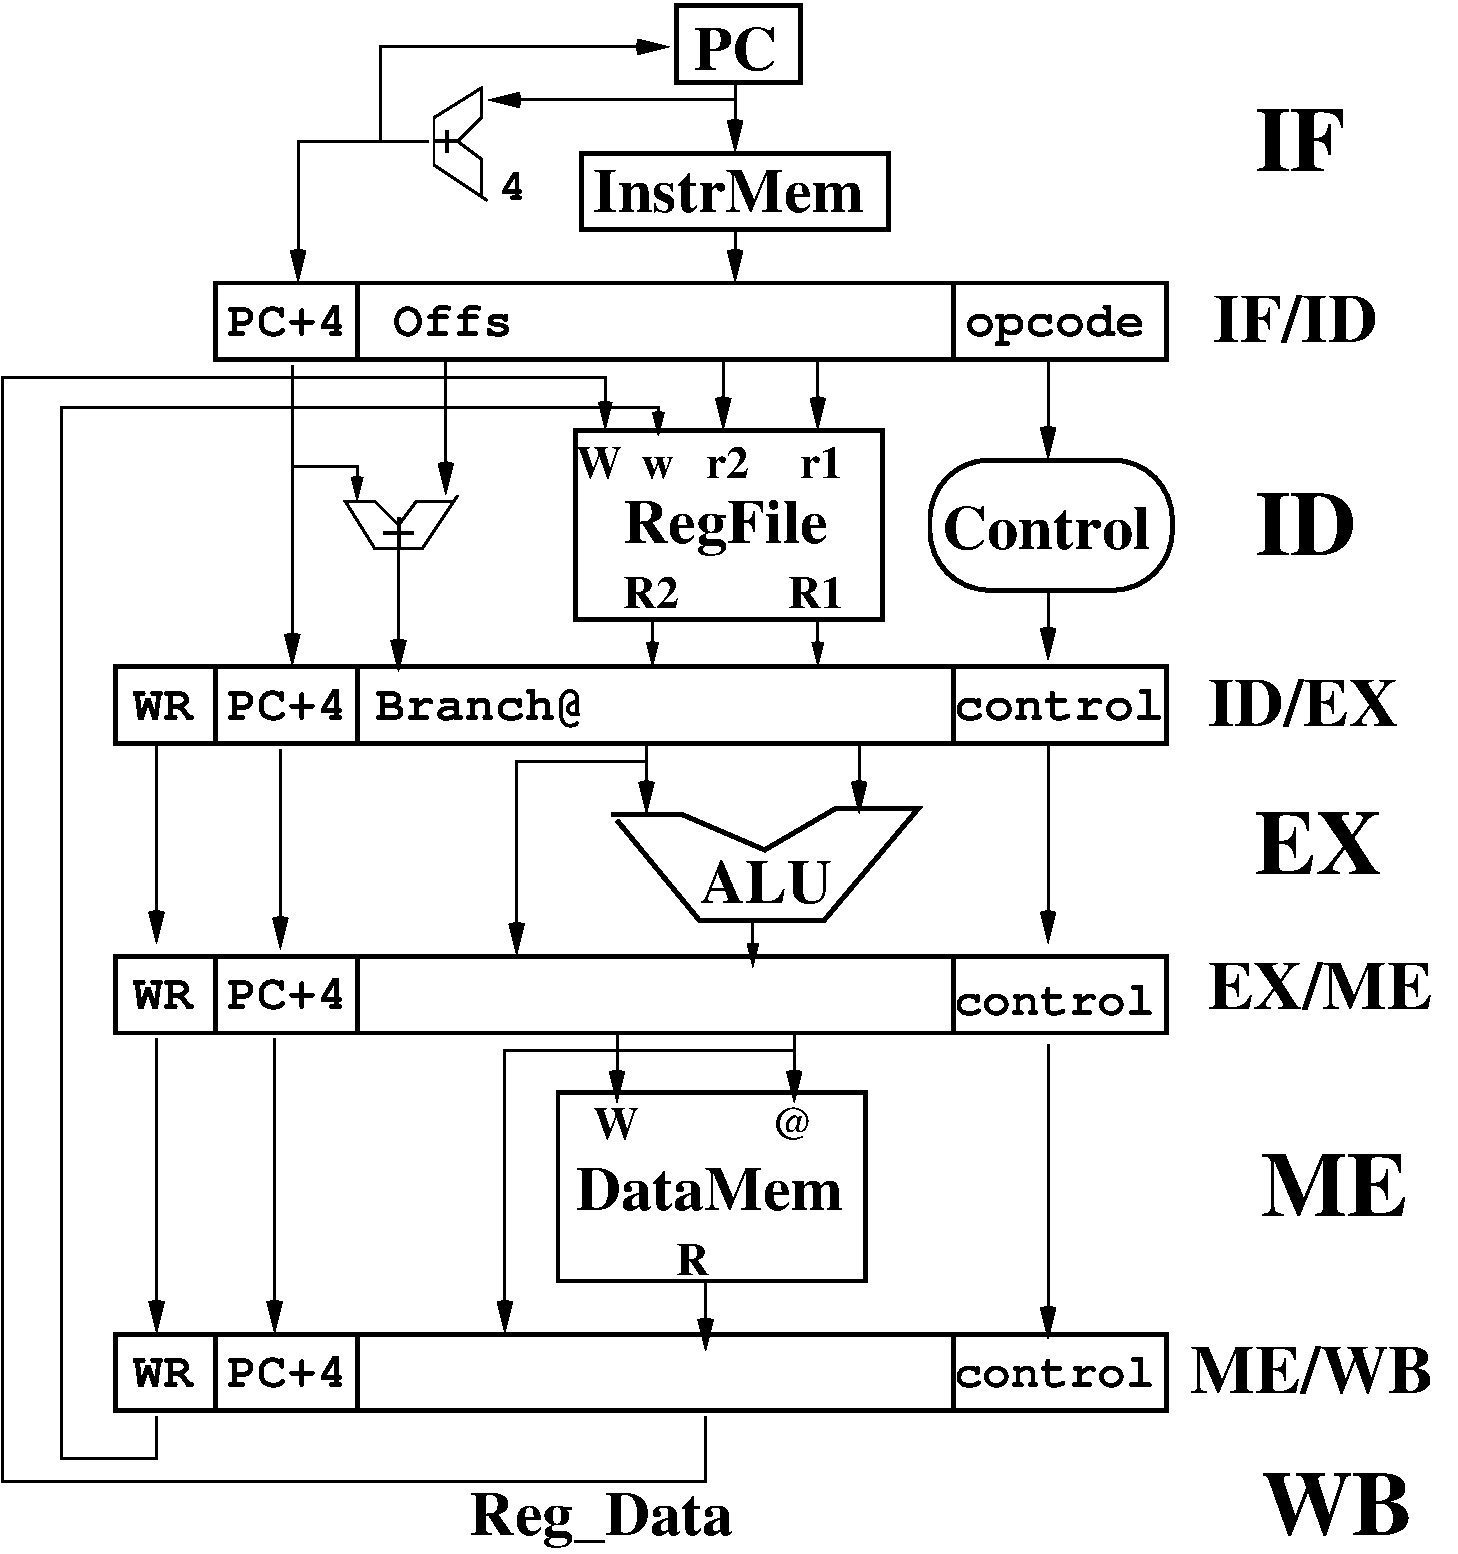
\includegraphics[width=37ex]{Figures/ClassicPipeline}
\end{columns}

\bigskip
\emp{This design assumes independent load, store, and ALU instructions},
i.e., instructions do not share registers or memory locations.
%Otherwise incorrect execution, because it does not account for data/control dependencies.

\end{frame}


\begin{frame}[fragile,t]
\frametitle{Classic RISC Pipeline Architecture}

\begin{columns}
\column{0.50\textwidth}
\begin{scriptsize}
\begin{itemize}
\item \emp{EX:} control signals of EX are applied and stripped. 
                One input reg connected to {\sc alu}. 2nd {\sc alu}
                input is either a register or, not shown, the 
                16 least significant digits (immed/displ).
                For load/stores {\sc alu} computes addresses.
                The value to store bypasses {\sc alu}.
\item \emp{ME:} control signals of ME are applied and stripped.
                For load/stores the address is the {\sc alu} output,
                and feeds into the address bus of the memory.
                The value to store connected to the input data bus.
                Values are stored/loaded from mem at trailing edge. 
                ALU instrs bypass ME stage.
\item \emp{WB:} remaining control signals applied. The mem value
                (for load) or from {\sc alu} is stored 
                to output register at the trailing edge of the clock.
                WR field used to index the register file.                 
\end{itemize}
\end{scriptsize}
\column{0.51\textwidth}\vspace{-2ex}
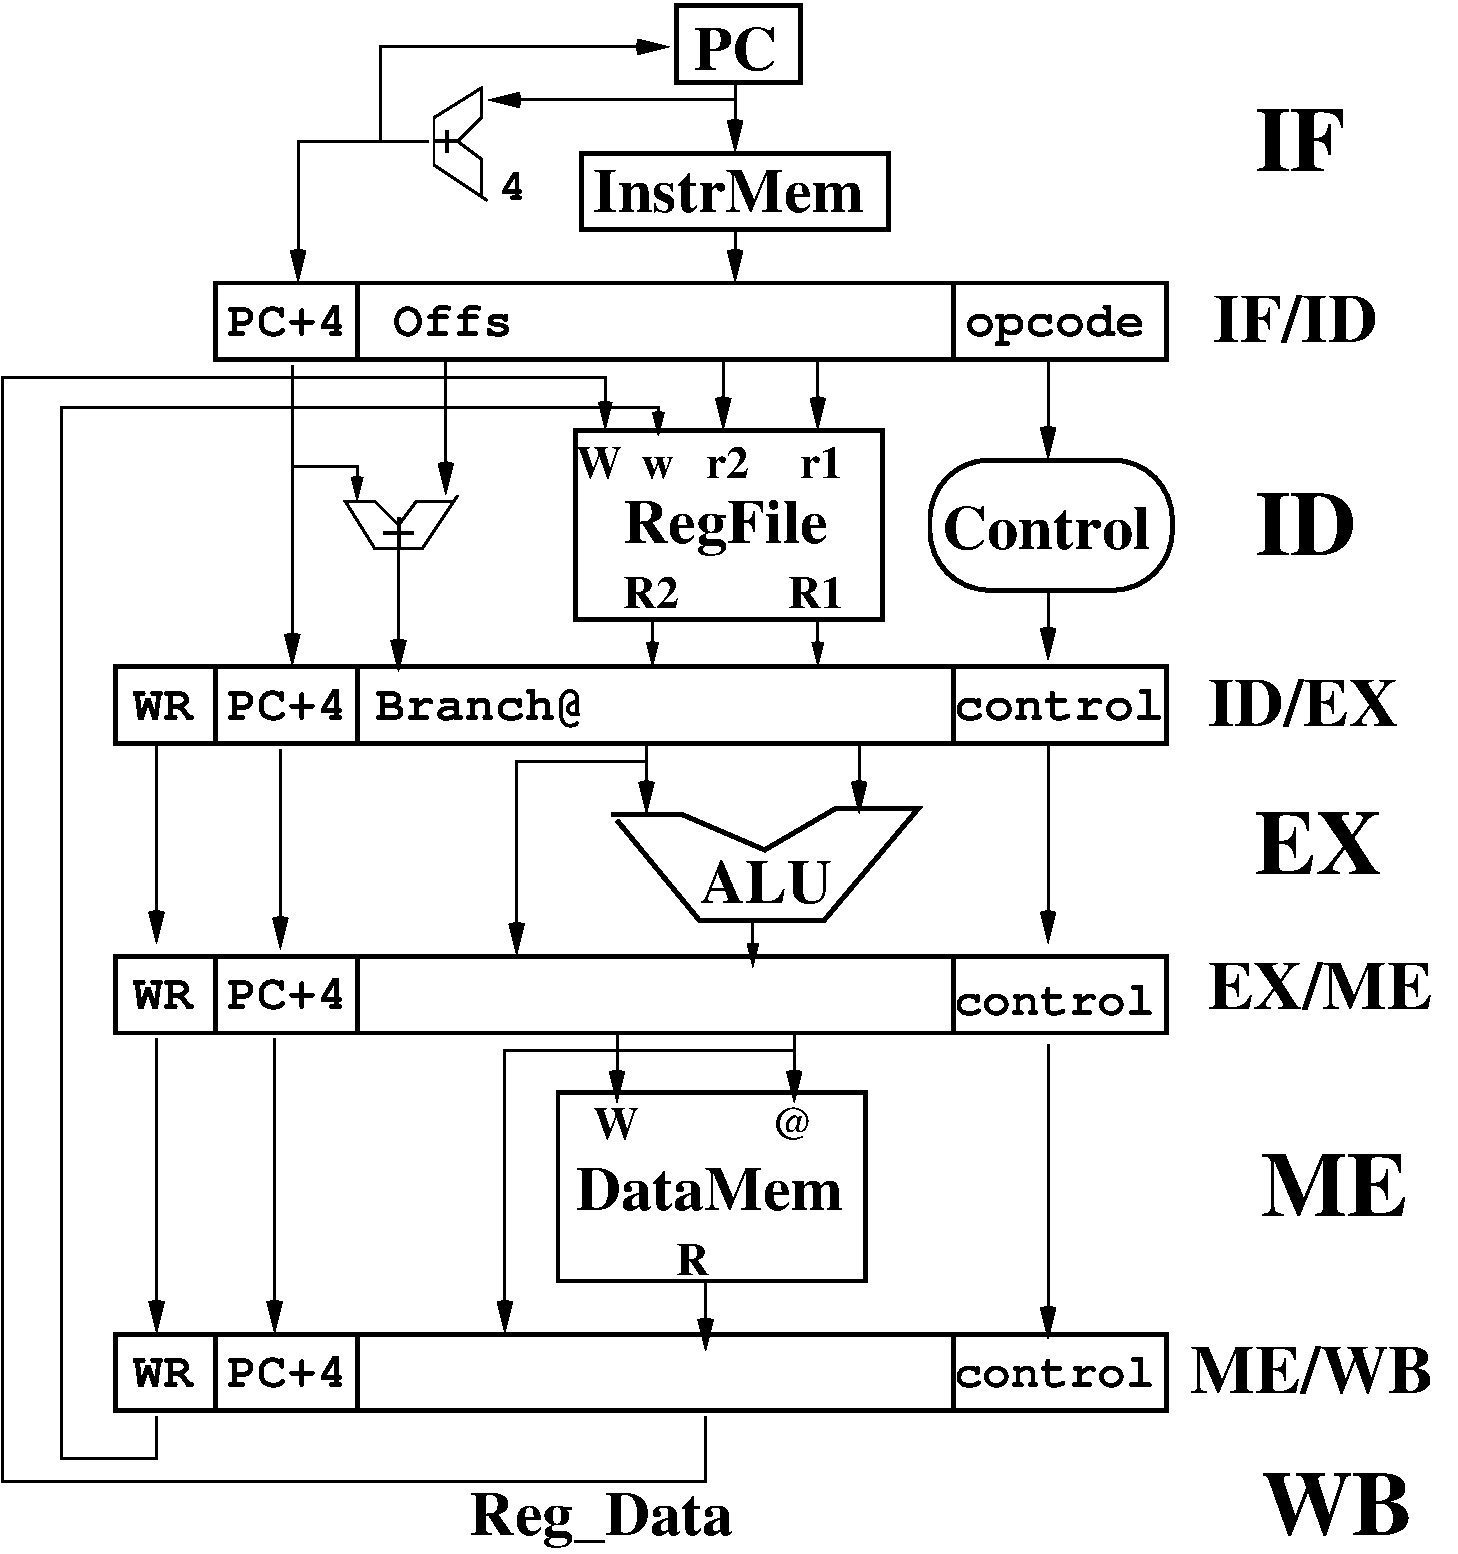
\includegraphics[width=37ex]{Figures/ClassicPipeline}
\end{columns}


\emp{This design assumes independent load, store, and ALU instructions},
i.e., instructions do not share registers or memory locations.
%Otherwise incorrect execution, because it does not account for data/control dependencies.

\end{frame}

\subsection{Resolving Data Hazards for the 5-Stage Pipeline}

\begin{frame}[fragile,t]
\frametitle{Data Hazards for the 5-Stage Pipeline}

\begin{block}{Data Hazards: Property of Software}
\begin{colorcode}
RAW (True Dependency)    WAR (Anti Dependency)    WAW (Output dependency)
S1    X  = ..            S1    .. = X             S1    X = ...            
S2    .. = X             S2    X  = ..            S2    X = ...
// S2; S1 gives a different result than S1; S2 => Hazard
\end{colorcode}
\end{block} 
\bigskip
\begin{scriptsize}
What hazards can occur in the 5-Stage Pipeline?
\begin{itemize}
\item \emph{Dependencies on memory operands} do not cause hazards 
        because loads/stores are executed in ME stage in program order.\smallskip
\item \emph{WAW hazards} are not possible because output-register is updated
        at the end of WB stage in program order. Same argument
        holds for \emph{WAR hazards}.\smallskip
\item \alert{RAW hazards are real!} Exercise: In the table below, which instrs cause hazards?
\end{itemize}
\end{scriptsize}
\bigskip
\begin{scriptsize}
\begin{tabular}{lllllllllll}
\hline
   & Clock$\Rightarrow$ & C1 & C2 & C3 & C4 & C5 & C6 & C7 & C8 & C9 \\\hline
I1 & ADD  R1,R2,R3      & IF & ID & EX & ME & WB &    &    &    &    \\
I2 & ADDI R3,R1,\#4     &    & IF & ID & EX & ME & WB &    &    &    \\
I3 & LW   R5,0(R1)      &    &    & IF & ID & EX & ME & WB &    &    \\
I4 & ORI  R6,R1,\#9     &    &    &    & IF & ID & EX & ME & WB &    \\
I5 & SUBI R1,R1,R7      &    &    &    &    & IF & ID & EX & ME & WB \\\hline
\end{tabular}
\end{scriptsize} 

\end{frame}


\begin{frame}[fragile,t]
\frametitle{RAW Data Hazard Example}

\bigskip

\begin{scriptsize}
\begin{tabular}{lllllllllll}
\hline
   & Clock$\Rightarrow$ & C1 & C2 & C3 & C4 & C5 & C6 & C7 & C8 & C9 \\\hline
I1 & ADD  R1,R2,R3      & IF & ID & EX & ME & WB &    &    &    &    \\
I2 & ADDI R3,R1,\#4     &    & IF & ID & EX & ME & WB &    &    &    \\
I3 & LW   R5,0(R1)      &    &    & IF & ID & EX & ME & WB &    &    \\
I4 & ORI  R6,R1,\#9     &    &    &    & IF & ID & EX & ME & WB &    \\
I5 & SUBI R1,R1,R7      &    &    &    &    & IF & ID & EX & ME & WB \\\hline
\end{tabular}
\end{scriptsize} 

\bigskip

\begin{scriptsize}
What hazards can occur in the 5-Stage Pipeline?
\begin{itemize}
\item I1 updates register R1 at the trailing edge of clock C5. \smallskip
\item All other instructions use (read) R1, hence potential hazards.
\item I5 reads R1 in ID stage in clock C6, after I1 has updated it in C5,
            hence RAW dependency is respected (\emph{I5 correctly reads the
            value produced by I1})\smallskip
\item All other instructions I2, I3, and I4 read R1 in ID stage sooner than
            end of clock C5 $\Rightarrow$ hence they all read a stale value 
            $\Rightarrow$ \alert{I2, I3, and I4 cause hazards}. 
\end{itemize}
\end{scriptsize}

\end{frame}

\begin{frame}[fragile,t]
\frametitle{Resolving RAW Hazards Generated by ALU Instr}

\bigskip

\begin{scriptsize}
\begin{tabular}{lllllllllll}
\hline
   & Clock$\Rightarrow$ & C1 & C2 & C3 & C4 & C5 & C6 & C7 & C8 & C9 \\\hline
I1 & ADD  R1,R2,R3      & IF & ID & EX & \emp{ME} & WB &    &    &    &    \\
I2 & ADDI R3,R1,\#4     &    & IF & ID & \emph{EX} & ME & WB &    &    &    \\
I3 & LW   R5,0(R1)      &    &    & IF & ID & \emph{EX} & ME & WB &    &    \\
I4 & ORI  R6,R1,\#9     &    &    &    & IF & ID & EX & ME & WB &    \\
I5 & SUBI R1,R1,R7      &    &    &    &    & IF & ID & EX & ME & WB \\\hline
\end{tabular}
\end{scriptsize} 

\bigskip

\begin{scriptsize}
\begin{itemize}
\item The hazard by I4 is solved by a small modification in the \emp{register file},
        named \emph{register forwarding}: if the same register is read and 
        updated in the same cycle then the updated value is forwarded to the
        reader. Easy to implement, requires several multiplexers to the 
        register file's ports.\smallskip
        
\item For the hazards by I2 and I3, observe that the {\tt R1} value
        is available at the end of C3, while I2 and I3 uses it at the
        beginning of C4 and C5, respectively.\smallskip

\item The new value (of {\tt R1}) can be \emph{forwarded to both ALU inputs}
\begin{itemize}
\begin{scriptsize}
        \item from \emp{register {\tt EX/ME}}, at the beginning of C4,
                thus solving the hazard of I2.\smallskip
        \item from \emp{register {\tt ME/WB}} (via {\tt REG\_data}), 
                at the beginning of C5, 
                thus solving the hazard of I3.\smallskip
\end{scriptsize}
\end{itemize}
\end{itemize}
\end{scriptsize}

\end{frame}


\begin{frame}[fragile,t]
\frametitle{Resolving RAW Hazard Generated by a Load}

\bigskip

\begin{scriptsize}
\begin{tabular}{lllllllllll}
\hline
   & Clock$\Rightarrow$ & C1 & C2 & C3 & C4 & C5 & C6 & C7 & C8 & C9 \\\hline
I1 & LW   R1,0(R3)      & IF & ID & EX & ME & \emp{WB}&    &    &    &    \\
I2 & ADDI R3,R1,\#4     &    & IF & ID & \alert{EX} & ME & WB &    &    &    \\
I3 & LW   R5,0(R1)      &    &    & IF & ID & \emph{EX} & ME & WB &    &    \\
I4 & ORI  R6,R1,\#9     &    &    &    & IF & \emph{ID} & EX & ME & WB &    \\
I5 & SUBI R1,R1,R7      &    &    &    &    & IF & ID & EX & ME & WB \\\hline
\end{tabular}
\end{scriptsize} 


\begin{scriptsize}
\begin{itemize}

\item The new value (of the load to {\tt R1}) is available at the end of C4 (end of ME).
\item Hazards of I3 and I4 are taken care by register-to-register forwarding,
\item \alert{It is not possible to forward the new value in time for I2}:
\begin{itemize}
\begin{scriptsize}
        \item because I2 needs it at the beginning of C4 in EX, during
                which the load accesses memory!
        \item \emph{This hazard need to be detected and I2 (and all following instructions)
                must be stalled as below} $\Rightarrow$ 1 cycle is lost.
\end{scriptsize}
\end{itemize}
\end{itemize}
\end{scriptsize}

\begin{scriptsize}
\begin{tabular}{lllllllllll}
\hline
   & Clock$\Rightarrow$ & C1 & C2 & C3 & C4 & C5 & C6 & C7 & C8 & C9 \\\hline
I1 & LW   R1,0(R3)      & IF & ID & EX & ME & \emp{WB}&    &    &    &    \\
I2 & ADDI R3,R1,\#4     &    & IF & ID & ID &\emph{EX} & ME & WB &    &   \\
I3 & LW   R5,0(R1)      &    &    & IF & IF & ID & \emph{EX} & ME & WB &   \\
I4 & ORI  R6,R1,\#9     &    &    &    &    & IF & \emph{ID} & EX & ME & WB\\
I5 & SUBI R1,R1,R7      &    &    &    &    &    & IF & ID & EX & ME       \\\hline
\end{tabular}
\end{scriptsize} 

\end{frame}

\begin{frame}[fragile,t]
\frametitle{Implementing Forwarding}

\begin{columns}
\column{0.51\textwidth}
\begin{scriptsize}
\begin{itemize}
\item Modifications are shown in \blue{blue}, dotted lines denote
            control lines.\bigskip
\item \emph{Operand Forwarding} uses one three-way multiplexer 
            to {\bf each} input of ALU, but only one is shown.
            \blue{\tt ForwardingMUX} selects between:\\
            (1) the ``normal'' value of {\tt ID/EX},\\ %(from the ID stage)
            (2) the ALU value, latched in {\tt EX/ME},\\
            (3) the WB value, latched in {\tt REG\_data}.\bigskip
           
\item \blue{Forwarding Unit} controls the 2 MUX:\\
            (1) Compares the {\tt WR} fields in {\tt EX/ME} and {\tt ME/WB} with
                 the \blue{input-register numbers} of the currently instr in EX.\\
            (2) If match selects {\tt EX/ME} or {\tt ME/WB},\\
            (3) Else selects {\tt ID/EX}, no hazard. 
\end{itemize}
\end{scriptsize}
\column{0.51\textwidth}\vspace{-2ex}
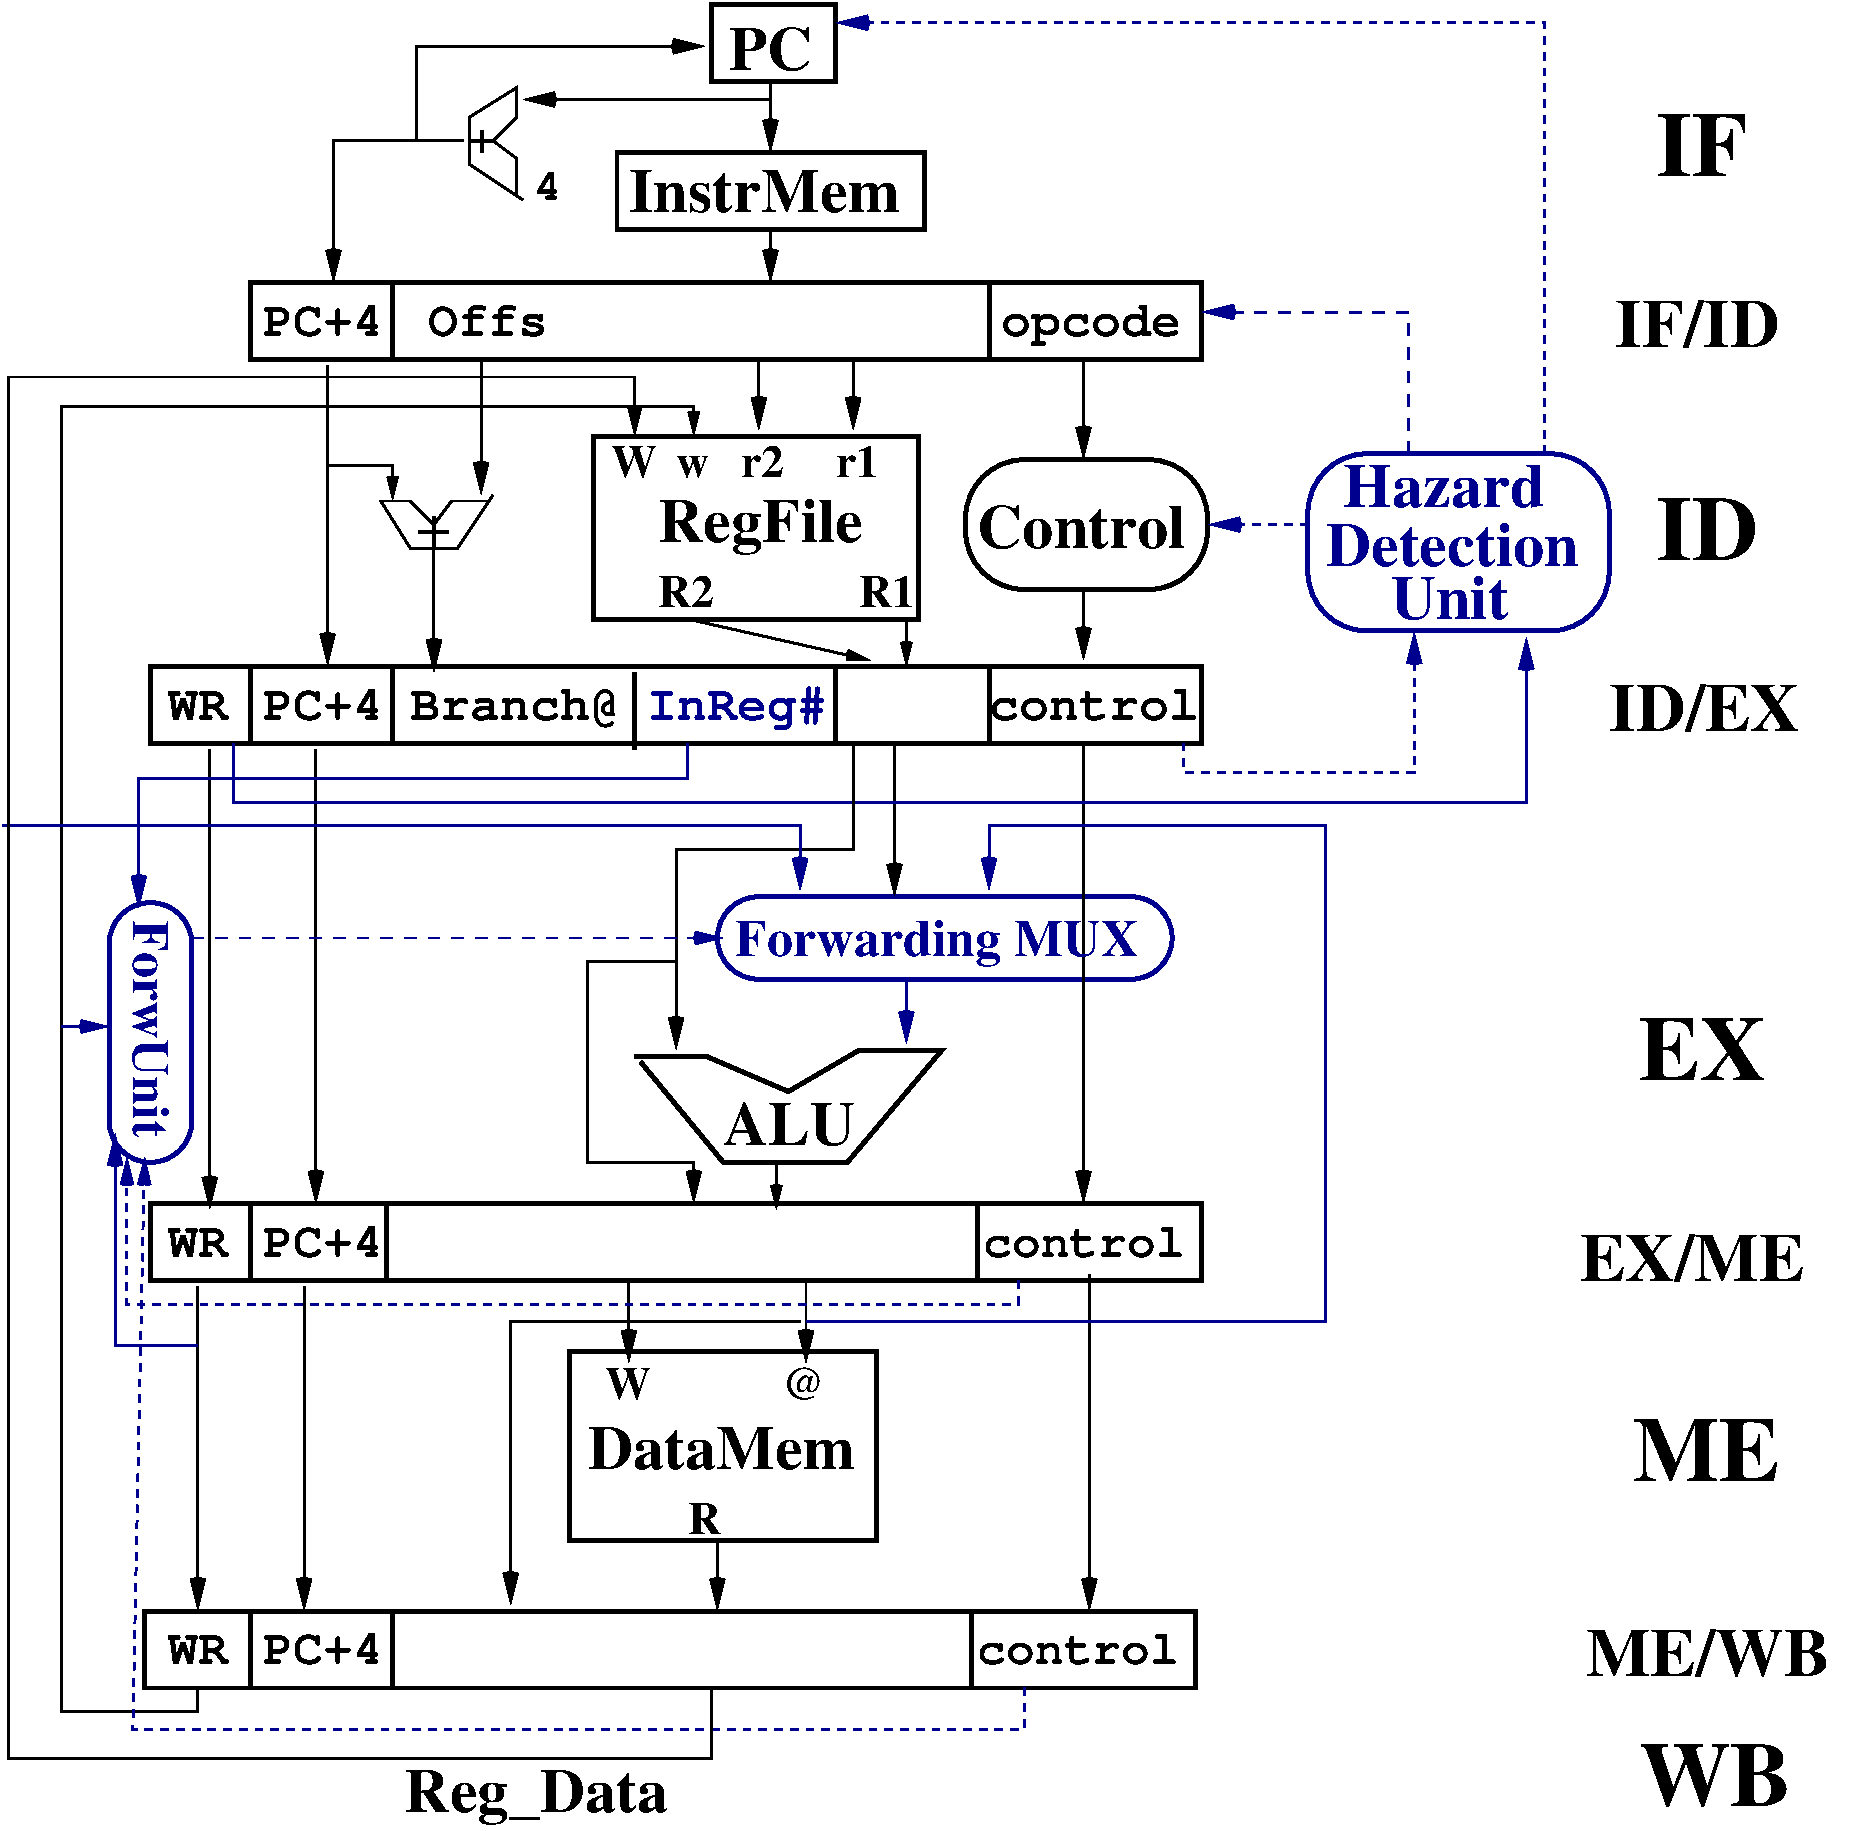
\includegraphics[width=37ex]{Figures/ClassicPipelineDH}
\end{columns}
\bigskip
\emph{Forwarding logic is simple}, \emp{the major complexity is 
to bus operand values across pipeline stages}.

\end{frame}

\begin{frame}[fragile,t]
\frametitle{Implementing Stalling}

\begin{columns}
\column{0.51\textwidth}
\begin{scriptsize}
\begin{itemize}
\item Modifications are shown in \blue{blue}, dotted lines denote
            control lines.\bigskip
\item \blue{Hazard Detection Unit (HDU)} \emph{stalls the pipeline} whenever
        a load is immediately followed by a dependent instr,\smallskip
\item It checks whether the instruction in EX is a load whose destination
        register is the same as one of the input registers of the 
        next instruction, i.e., the one in ID.\smallskip
\item If so then HDU \emph{stalls} the IF and ID stages 
        and propagates a NOOP to EX stage. Accomplished 
        by disabling the clock of PC, IF and ID.
\end{itemize}
\end{scriptsize}
\column{0.51\textwidth}\vspace{-2ex}
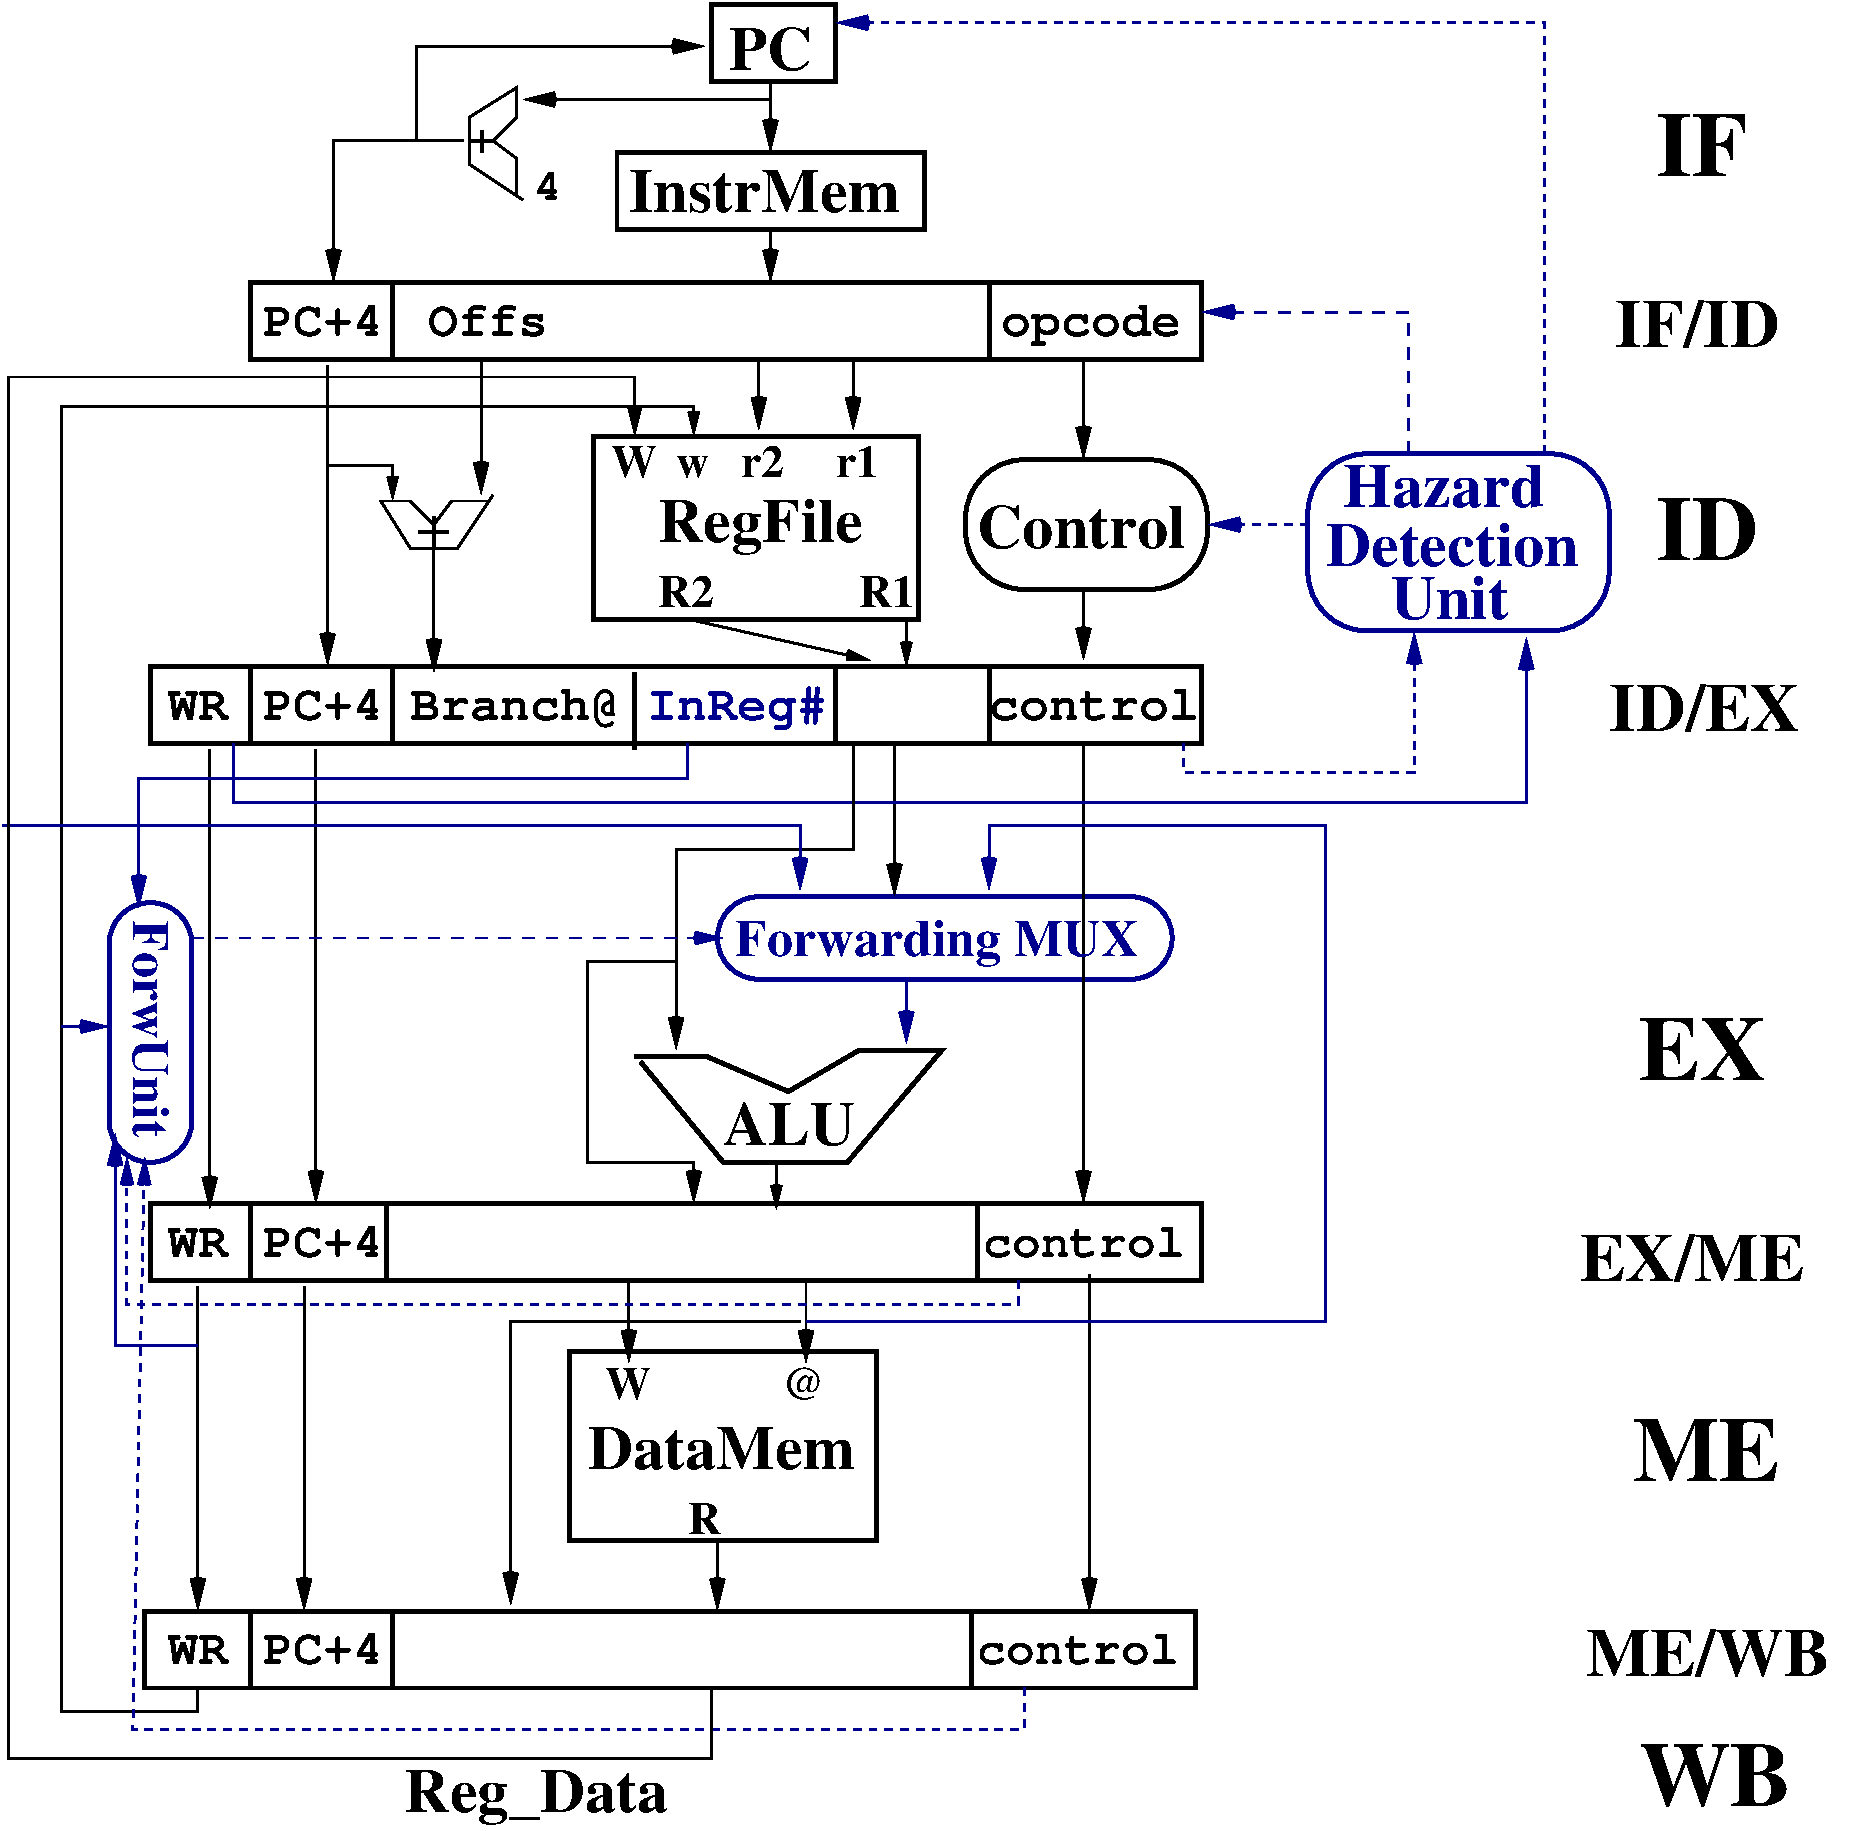
\includegraphics[width=37ex]{Figures/ClassicPipelineDH}
\end{columns}

\bigskip

\emph{Stalling is simpler than forwarding, since no operand value is bussed},
but also \emp{less efficient, since one clock is lost.}

\end{frame}

\subsection{Resolving Control Hazards for the 5-Stage Pipeline}

\begin{frame}[fragile,t]
\frametitle{Resolving Control Hazards}

\begin{columns}
\column{0.51\textwidth}
\begin{scriptsize}
\begin{itemize}
\item \emp{A branch} is assumed not taken until the end of EX, 
        when its condition was evaluated by {\sc alu}.
        (Target address is computed in ID.) If {\sc alu}'s 
        \blue{\tt Z} bit is set $\Rightarrow$ branch taken by 
        performing 2 actions:
\item[1] Target address is latched into PC at the end of cycle.
        If \blue{\tt Z}=1 (and instr in EX is a branch) then 
        \blue{MUX} feeding into PC selects the branch target.
\item[2] IF and ID stages must be flushed.  This is done by
            \blue{Control} when its input is 1, by zeroing out
            the control fields.
\item \emp{Jumps with absolute addresses} are taken at the end of IF.
\item \emp{Indirect jumps} ({\tt JR}) are taken at the end of ID,
         because register containing the target address must
        be fetched $\Rightarrow$ instr in IF must be flushed.
%target address is latched into PC

%        and also the operand values
%        might depend on previous instructions. Same for {\tt JR}. 
\end{itemize}
\end{scriptsize}
\column{0.51\textwidth}\vspace{-2ex}
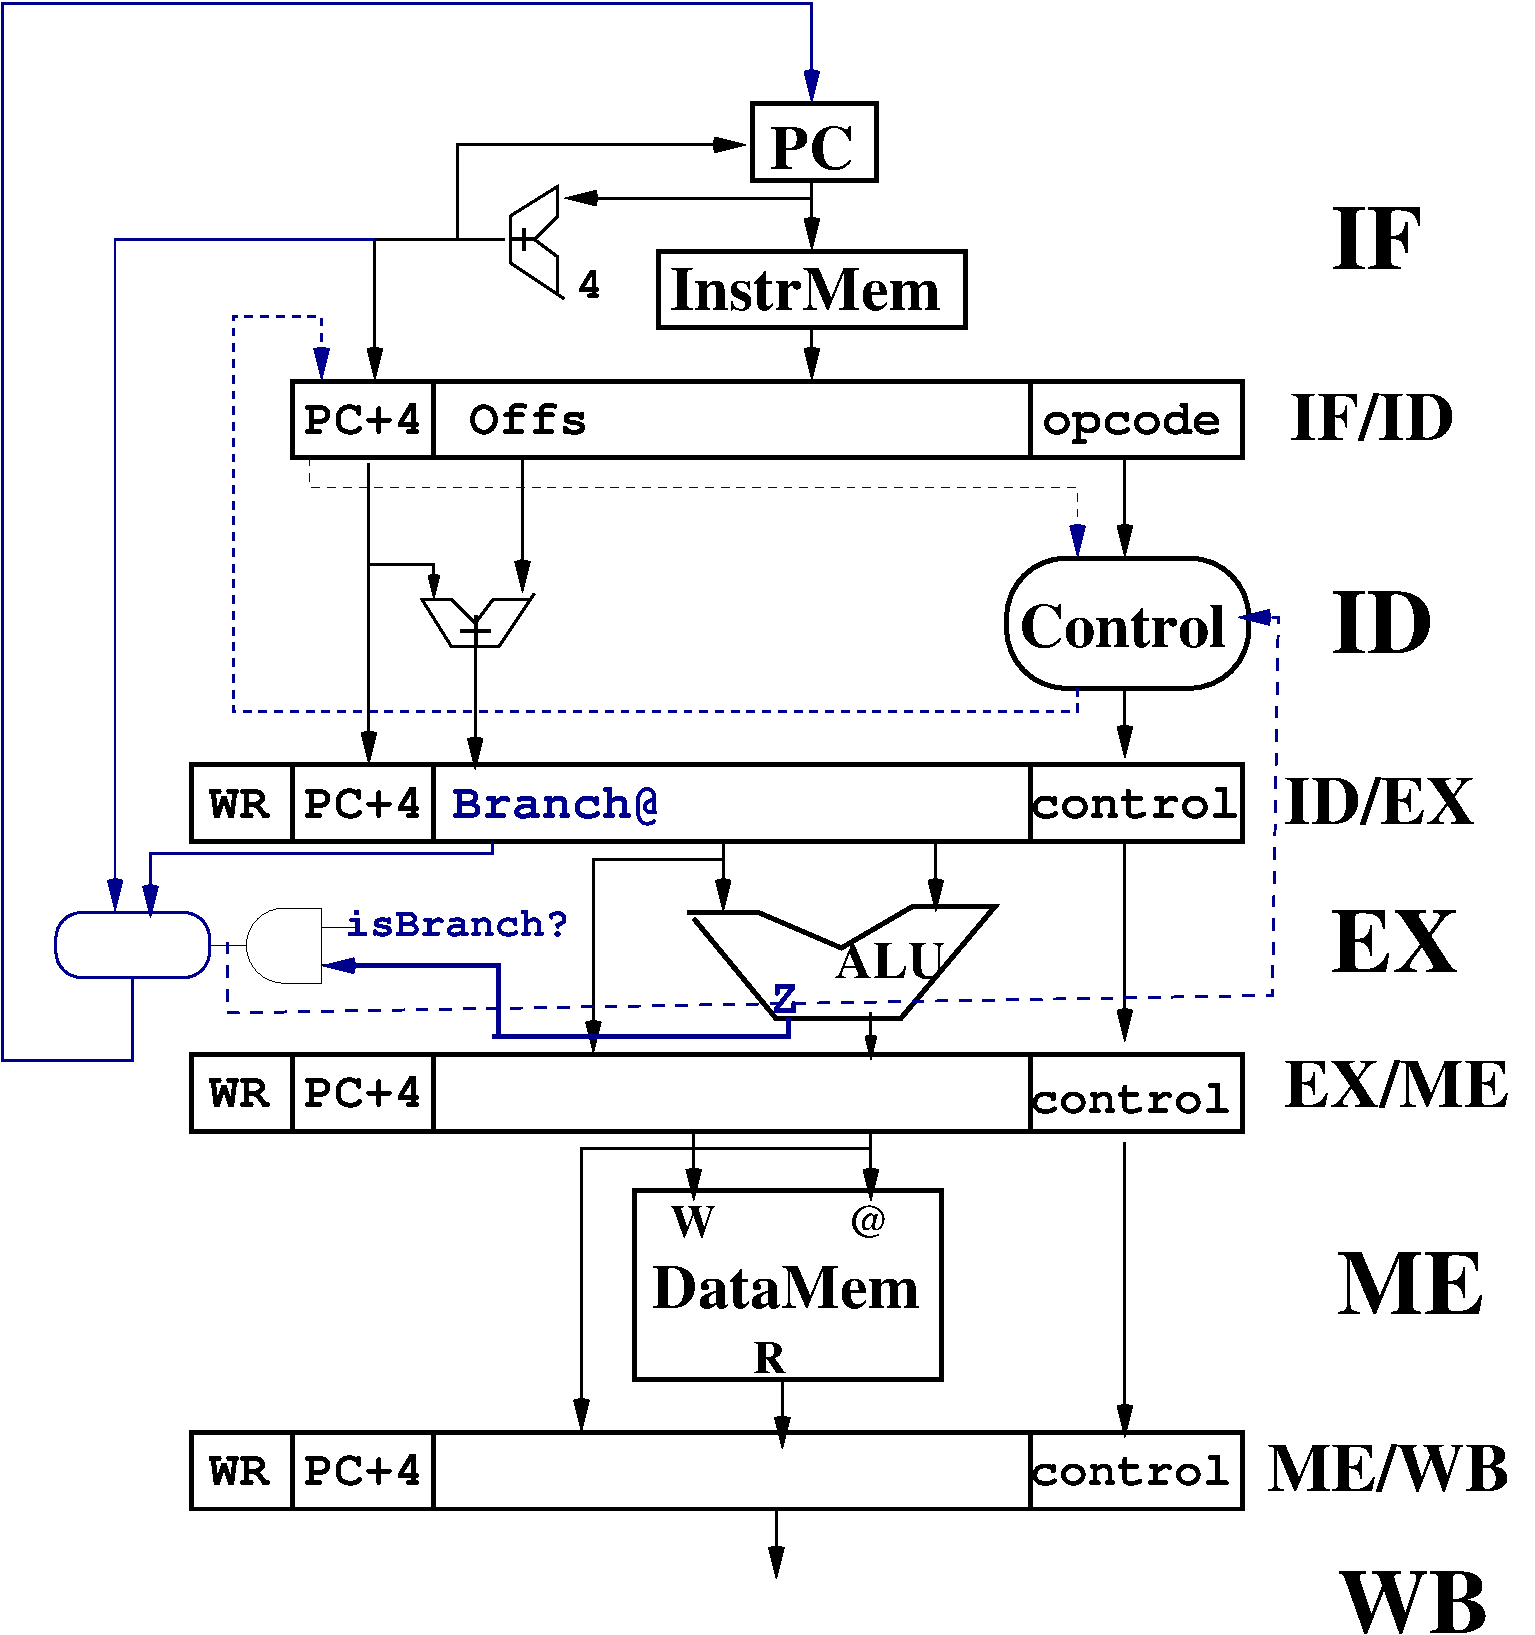
\includegraphics[width=37ex]{Figures/ClassicPipelineCF}

\blue{Modifications are colored blue}.
\end{columns}

\bigskip

\emp{Two cycles are lost on a taken branch, and one on an indirect jump.}

\end{frame}

\subsection{Handling Precise Exceptions in the 5-Stage Pipeline}

\begin{frame}[fragile,t]
\frametitle{Structural Hazards \& Precise Exceptions}

\begin{scriptsize}
\begin{itemize}
\item 5-stage pipeline exhibits \emph{NO structural hazards!} 
        (conflicts to shared resources).\bigskip

\item \emp{Precise exceptions} may be triggered in all stages but WB,
        e.g., page fault in IF/ME, undefined instr in ID, and
              arithmetic overflow in EX. Whenever they occur:
\item[1] faulting \& following instructions are squashed,
\item[2] all instructions preceding the faulty one must complete,
\item[3] execution of exception handler must start.\bigskip

\item \emp{However, taking the exception in the same cycle it occurs is very complex:}
\item[1] to-be-flushed stages depend on the stage in which exception occurred,
% exception condition and PC must be accessible to treat the exception
% and they reside in different stages.
\item[2] multiple exceptions may occur in the same cycle in different stages, and
\item[3] exceptions must be taken in program order,
            e.g., page faults occurring in IF, but later, a 
            preceding instruction in EX causes another
            exception.\bigskip
 
\item \emp{A Radical Solution is to flag an exception but keep
            it silent until instr reaches WB}.
            The first exception on an instr is recorded in an
            exception-status register (ESR) and the instr is NOOPed. 
            (ESR is carried through the whole pipeline.)
            Exceptions are taken in WB stage, hence in program order.
\item \alert{One issue is that a store in ME must be disabled
                if the preceding instr takes an exception} 
                $\Rightarrow$ requires additional hardware.   
 
%target address is latched into PC

%        and also the operand values
%        might depend on previous instructions. Same for {\tt JR}. 
\end{itemize}
\end{scriptsize}
\end{frame}

\section{Out-Of-Order Instruction Completion}

\begin{frame}[fragile]
	\tableofcontents[currentsection]
\end{frame}

\subsection{Data, Control, Structural Hazards \& Exceptions}

\begin{frame}[fragile,t]
\frametitle{Out-Of-Order Instruction Completion: Data Hazards}

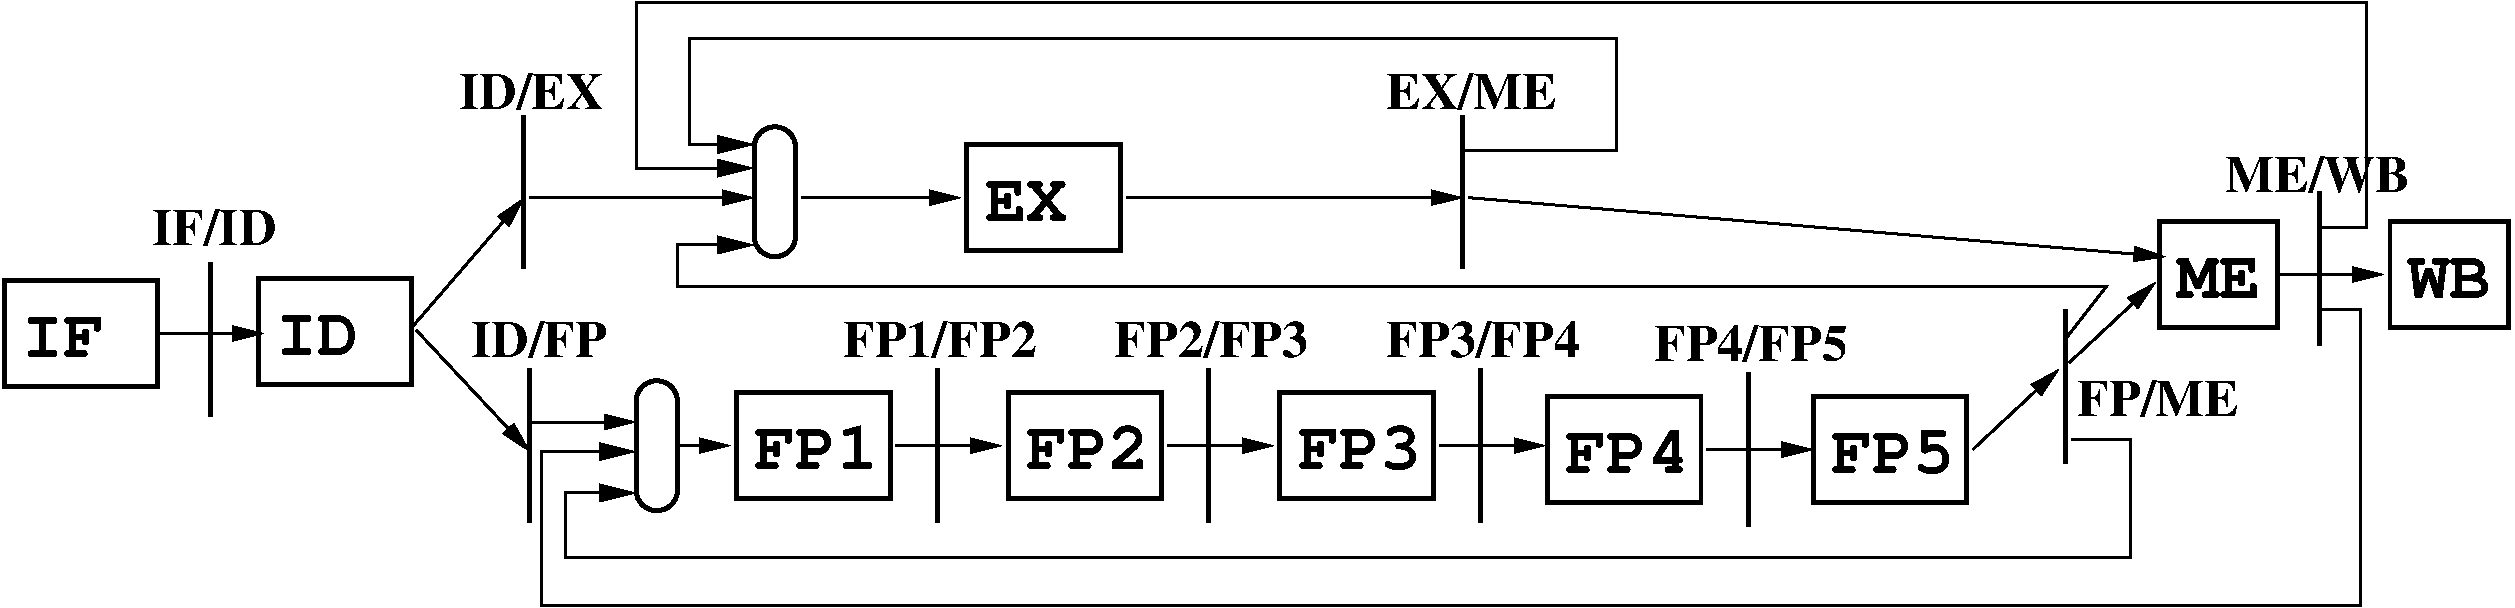
\includegraphics[width=59ex]{Figures/SimpleOoOPipeline}

\bigskip

\begin{scriptsize}
\begin{itemize}
\item Based on instr's {\tt opcode} the decoder sends an instr
        either on the integer (load/store/ALU/branches) or 
        floating-point pipeline,
        but all instr go through ME and WB stages.
        Machine has two separate register files, integer \& float.\bigskip

\item \emp{Data Hazards:} 
\item[1] \emp{Forwarding is more complicated} because float stores need the
            values of both an integer address and a float register $\Rightarrow$
            \emph{a forwarding path was added from {\tt FP/ME} to the
                    input of EX}.\smallskip
\item[2] \emp{Hazard Detection Unit (HDU) is more complicated} because both RAW and WAW
            hazards are possible. HDU must stall instrs in ID stage if they
            have register dependencies with a preceding instruction 
            $\Rightarrow$ \emph{source \& destination registers 
            of an instr in ID are checked against ALL destination registers
            of instrs in execution}.\smallskip
\item[3] Data hazards on memory operands \emph{NOT possible} because all
                instructions move through ME in program order.
\end{itemize}
\end{scriptsize}
\end{frame}


\begin{frame}[fragile,t]
\frametitle{Metrics: Latency of Operation \& Initiation Interval}

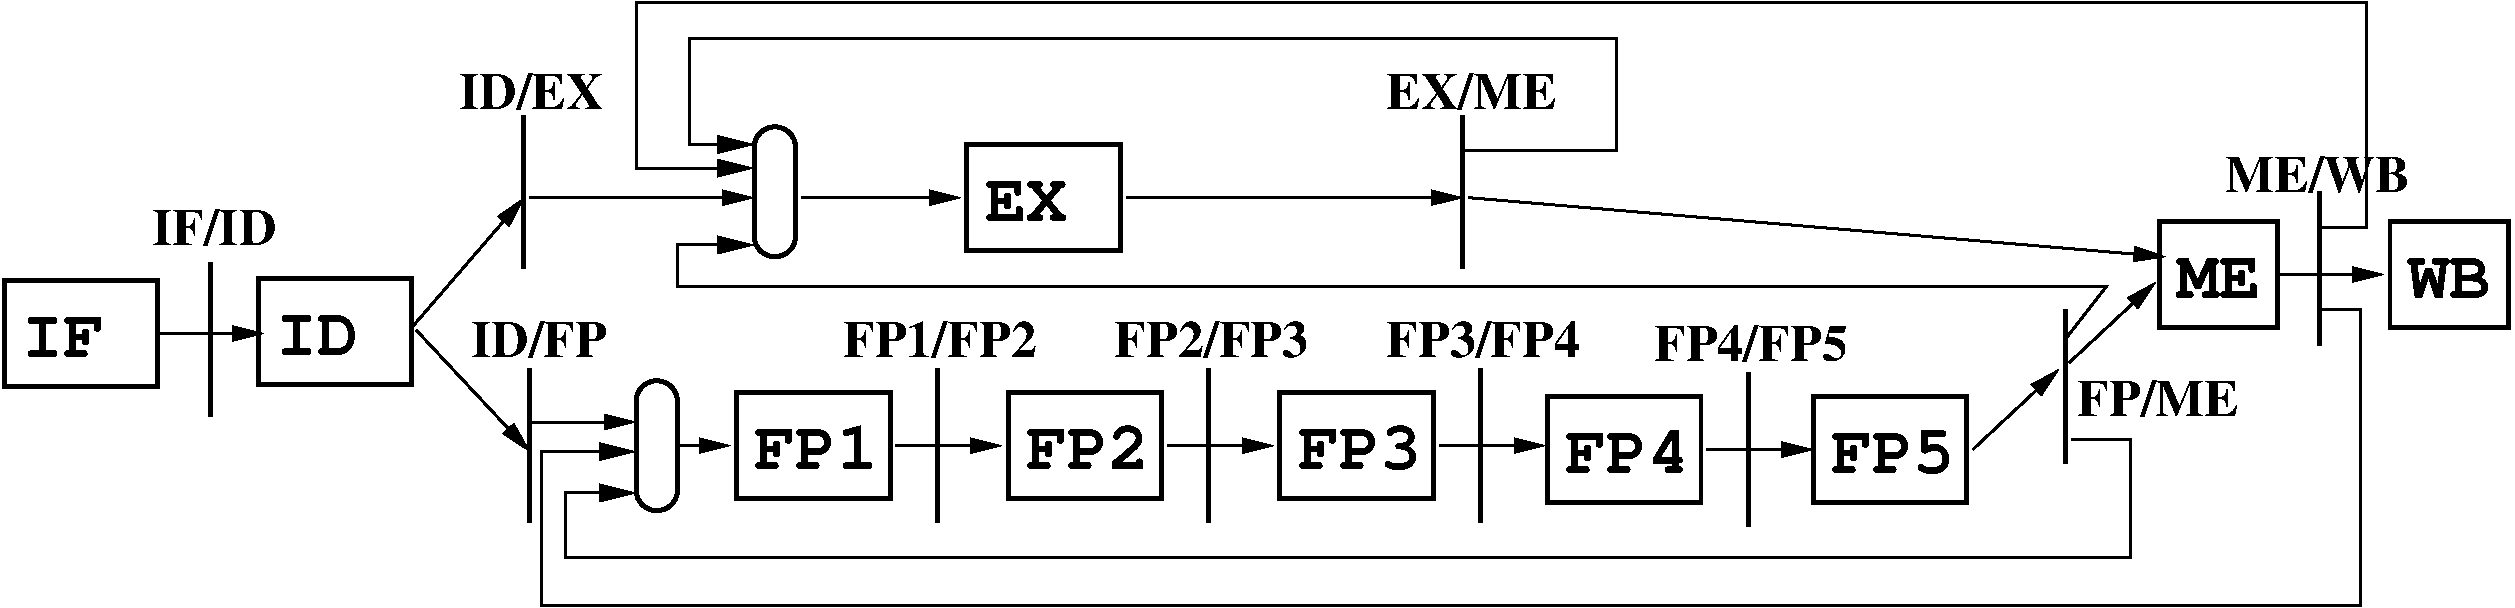
\includegraphics[width=53ex]{Figures/SimpleOoOPipeline}

\bigskip

\begin{scriptsize}
\begin{itemize}
\item \emp{Latency of Operation} of an instruction is the max \# of clocks 
        that the next instruction has to wait (in ID) to avoid a data hazard 
        ({\sc raw}/{\sc waw}).\smallskip
\item For the pipeline above: it is 1 for Load, and for the rest it is 
        (\# of clocks of EX - 1) because closest fwd is at the end of EX. 

\item Latency of FP unit is large (4) $\Rightarrow$ stalls are more frequent than in 5-stage pipeline:
\end{itemize}

\begin{tiny}
\begin{tabular}{lllllllllllll}
\hline
   & Clock$\Rightarrow$ & C1 & C2 & C3 & C4 & C5 & C6 & C7 & C8 & C9 & C10 & C11            \\\hline
I1 & L.D    F4,0(R2)     & IF & ID & EX & ME & \emp{WB} &    &    &    & & &                \\
I2 & MULT.D F0,F4,F6     &    & IF & ID & ID & \emph{FP1} & FP2 & FP3 & FP4 & FP5 & \emp{ME} & WB \\
I3 & S.D    F0,0(R2)     &    &    & IF & IF & ID & ID & ID & ID & ID & \emph{EX} & ME  \\\hline
\end{tabular}
\end{tiny}
\bigskip

\begin{itemize}
\item \emp{Initiation Interval} is the min \# of cycles between issuing 2 instrs
            of the same type to execution units.\smallskip
\item In our case is 1 because both integer and float units are fully pipelined,
        and linear. If float unit would not be pipelined, it would be 5.
      For dynamically scheduled pipelines it might be variable, 
        i.e., depending on what instructions were previously issued.
\end{itemize}
\end{scriptsize}
\end{frame}

\begin{frame}[fragile,t]
\frametitle{Control \& Structural Hazards}

\bigskip

\begin{scriptsize}
\begin{itemize}
\item \emp{Control Hazards} solved similarly as in static, 5-stage pipeline.\smallskip
\item \emp{Structural Hazards}: separate integer and float register files, BUT
        a float load/store may reach WB stage in the same cycle as a preceding
        float arithmetic instr $\Rightarrow$ structural hazard \emp{on the write port 
        of FP register file}.   \emph{This is possible because FP instrs in ME use
        a bus that bypasses memory $\neq$ from the bus of integer instrs.}  
\end{itemize}
\bigskip

\begin{tiny}
\begin{tabular}{llllllllllll}
\hline
   & Clock$\Rightarrow$ & C1 & C2 & C3 & C4 & C5 & C6 & C7 & C8 & C9 & C10            \\\hline
I1 & ADD.D F2,F4,F2     & IF & ID & FP1 & FP2 & FP3 & FP4 & FP5 & ME & \alert{WB} &      \\
I2 & ADD.D F6,F4,F6     &    & IF & ID & FP1 & FP2 & FP3 & FP4 & FP5 & ME & WB   \\
I3 & L.D   F8, 0(R1)    &    &    & IF & ID  & EX  & ME  & WB  &     &    &      \\
I4 & L.D   F10,0(R2)    &    &    &    & IF  & ID  & EX  & ME  & WB  &    &      \\
I4 & L.D   F14,0(R3)    &    &    &    &     & IF  & ID  & EX  & ME  & \alert{WB} &      \\\hline
\end{tabular}
\end{tiny}
\bigskip

\begin{itemize}
\item I1 and I5 being both in ME at C8 \emph{is Not a problem} 
        because I1 does not access memory. But in the next clock 
        \emp{both instrs write the FP register} file.\smallskip
\item Can be solved by stalling one of the instrs in ID, or by providing two write ports to
        the floating point register file.
\end{itemize}
\end{scriptsize}
\end{frame}


\begin{frame}[fragile,t]
\frametitle{Precise Exceptions in OoO Linear Pipelines}

\begin{scriptsize}
\begin{itemize}
\item \emp{Major Drawback} of OoO pipelines is that precise exceptions are hard
            to implement, e.g., because instrs reach WB stage out of order.
            
\item \emp{Sometimes not implemented}: hardware signals the software handler that
            an exception happened around some PC counter. This is not possible
            for page faults and strict FP standards (IEEE).\smallskip
\item Conservative technique of stalling in ID until all previous instrs
        are free of exceptions may stifle pipelining.\smallskip

\item Architecture can be modified to force in-order traversal of WB stage,
        hence exception can be taken in program order as in static 5-stage 
        pipeline, but at the cost of additional forwarding, and in addition
        a store can be issued only when all preceding instr are certified 
        free of exceptions. 
\end{itemize}
\end{scriptsize}
\end{frame}

\subsection{SuperPipelined and SuperScalar CPUs}

\begin{frame}[fragile,t]
\frametitle{Superpipelined CPU}

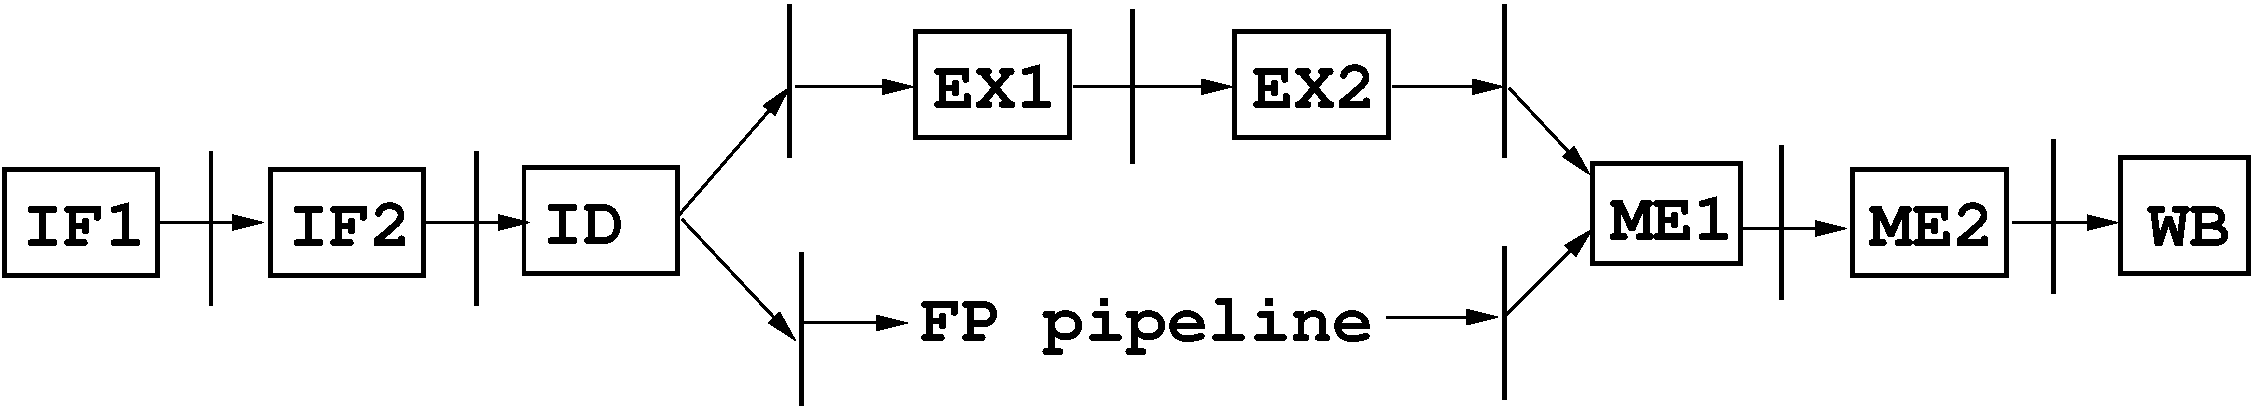
\includegraphics[width=59ex]{Figures/SuperPipeline}

\bigskip

\begin{scriptsize}
\begin{itemize}
\item In a given technology, some of the 5 stages have more delays than others.
        For example I-cache access in IF may take twice as decoding.
        Same with ME, because virtual-mem address translation in TLB is 
        done before accessing the data cache.\smallskip

\item \blue{CPU is superpipelined} when one of the 5 stages is further pipelined.\smallskip

\item It is also possible to pipeline every single stage (of the 5) to increase
            throughput.\bigskip

\item \blue{\em Superpipelines are clocked faster than the worst-case delay 
            of the bottleneck stage of the 5-stage pipeline}.
        \emph{Cycle time decreases,} \emp{but CPI increases} 
        $\Rightarrow$ no free lunch!\bigskip

\item For example, branches are executed in EX1 and have penalty 3.
\item Latency (of operation) of loads is 3.
\item Latency of register-to-register instructions is 1 (\# of EX stages-1).
\end{itemize}
\end{scriptsize}
\end{frame}

\begin{frame}[fragile,t]
\frametitle{Superscalar CPU}

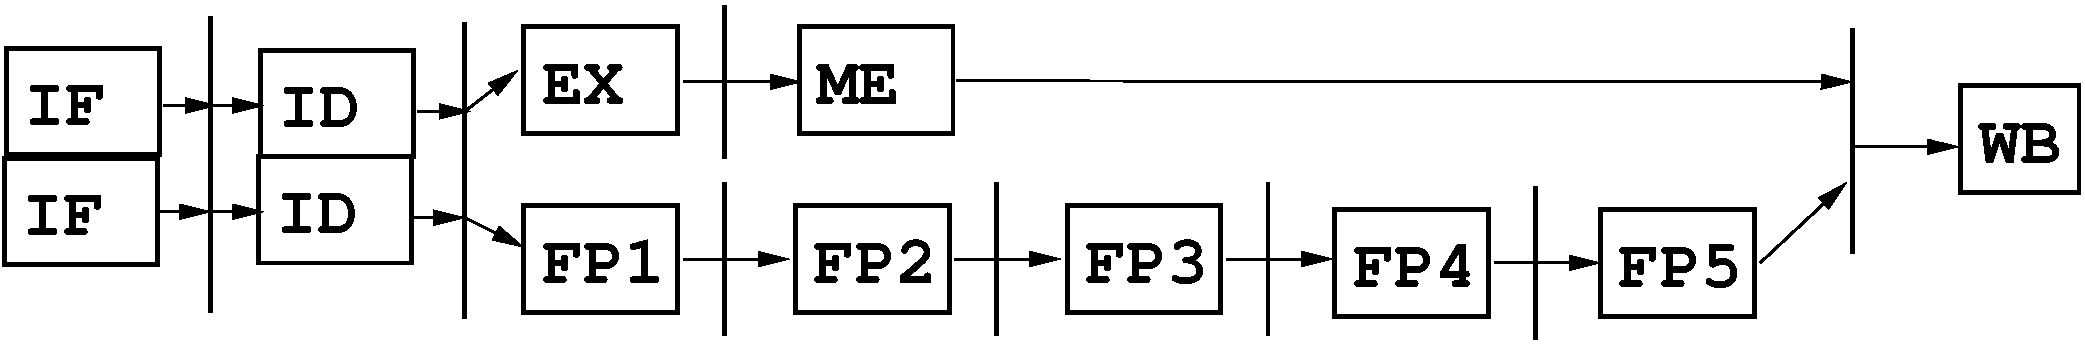
\includegraphics[width=59ex]{Figures/SuperScalar}

\bigskip

\begin{scriptsize}
\begin{itemize}
\item More than one instruction is fetched, decoded and issued in each cycle:

\item works well on workloads with a good mix of integer and float operations.\smallskip

\item \emph{With the above arch, up to two instrs (one int and one float) can proceed
        to execution once they are free of hazards $\Rightarrow$ CPI < 1}\bigskip

\item \emp{Supporting precise exceptions is difficult}.
\item \emp{Difficult to build static superscalars wider than 2 ways (int-float)},
\item e.g., integer pipeline could be split into three pipelines 
        (integer ALU, branches, memory) but such an architecture was never built!\bigskip
\end{itemize}
\end{scriptsize}

In practice superscalars may be superpipelined as well!

\end{frame}

\subsection{Branch Prediction}

\begin{frame}[fragile,t]
\frametitle{Branch Prediction}

\emp{Hardwired Prediction} is the most static algorithm and out of compiler's control.
\begin{scriptsize}
\begin{itemize}
\item always predict branch untaken $\Rightarrow$ no penalty when branch is untaken,
        but loop backedge misspredicted most of the time.\smallskip
\item predict based on {\tt opcode} \& direction/size of the address offset of the 
        branch instr
\item[1] {\tt BNEZ/BEZ} is predicted untaken/taken
\item[2] backward branches predicted as taken and forward as untaken
\item[3] branches with large offsets predicted as taken 
\item \emp{Prediction alg. is made at $\mu$architecture design time based on 
            a mix of benchmarks}.
\end{itemize}
\end{scriptsize}

\bigskip

\emp{Compiler-Guided Prediction}
\begin{scriptsize}
\begin{itemize}
\item Uses code profiling to determine the best prediction
        for each static branch in the code \& is communicated to hardware 
        by one extra bit in the branch instr format.
\item Note that if a branch is only taken for the first half of prg exec,
        and untaken for the second half, the compiler will predict it biased (50-50). 
\end{itemize}
\end{scriptsize}

\bigskip

For the studied architectures, target address is known only at the end of ID $\Rightarrow$
instrs in earlier stages must be flushed if branch is predicted taken, even when 
prediction is correct!

\end{frame}

\subsection{Strength \& Weaknesses of Static Pipelining}

\begin{frame}[fragile,t]
\frametitle{Strength \& Weaknesses of Static Pipelining}


\begin{scriptsize}
The studied (static) pipelines schedule instrs in the strict order 
dictated by compiler (while dynamic archs reorder instrs at runtime 
to optimize delays/stalls). {\bf Static Pipelines:} 
\begin{itemize}
\item[+] are \emph{simple} $\Rightarrow$ (1) better clock rate,
            (2) predictable performance, (3) consume less power since
                dynamic activities are migrated to the compiler.
\item[-] \emp{weak on dynamic events} such as conditional branches,
            exceptions, cache misses. 
        For example, the only way to deal with cache misses is to freeze
            the processor, refill the cache, \& replay cycle $\Rightarrow$
            only one mem access can proceed at any one time
            $\Leftarrow$ \emph{Alleviated by core multi-threading.}
\item[-] \emp{Static instr scheduling is limited by lack of dynamic info},
            such as memory addresses, e.g., do {\tt a[b[i]]} and 
            {\tt a[b[i+1]]} refer to the same element of {\tt a}?
\item[-] \emp{Precise exceptions are hard to handle efficiently} if OoO
            instr completion is allowed.
\item[-] \emp{The design of static pipelines might not scale well}, 
            i.e., as pipelines becoming deeper
            and wider (instr issuing), latencies $\uparrow$ and the
            compiler might solve them efficiently.  
\end{itemize}

\bigskip
\end{scriptsize}

\begin{itemize}
\item Static pipelines favored in embedded systems (simplicity),
\item Dynamic pipelines, studied towards the end of the course, are/were used
        in general-purpose environments,
\item \emph{Trend might reverse due to the advent of core multi-threading}.  
\end{itemize}

\end{frame}

%%%%%%%%%%%%%%%%%%%%%%%%%%%%%%%%%%%%%%%%%%%
%%%%%%%%%%%%%%%%%%%%%%%%%%%%%%%%%%%%%%%%%%%

\section{Core Multi-Threading}

\begin{frame}[fragile]
	\tableofcontents[currentsection]
\end{frame}

\begin{frame}[fragile,t]
\frametitle{Core Multi-Threading Overview}

\begin{scriptsize}
Operating System:
\begin{itemize}
\item Resources are precious \& expensive $\Rightarrow$ 
            better utilized by time multiplexing (sharing) them over a 
            number of concurrent processes, 
            $\Rightarrow$ $\uparrow$ process throughput.\smallskip
\item An active process is \emp{running or ready or blocked} 
            on a long latency IO (page fault).\smallskip
\item {\tt running $\rightarrow$ blocked/ready} and 
      {\tt ready $\rightarrow$ running} transitions
        involve context switching (100s of cycles overhead).
        Implemented entirely in software (flexibility).
\end{itemize}

\bigskip

Core Multi-Threading
\begin{itemize}
\item Same idea, but hides much smaller latencies,
        e.g., level-1/2/3 cache misses, TLB misses, long-latency instrs
                (co-processor), unsuccessful thread synch, etc.\smallskip
                % exceptions %and simplifies exception handling. 

\item Motivated by the ever increasing memory wall \& underutilization of 
        functional units (1990s), requires little to no modification of Operating System.

\item Each thread runs in a \emp{\em hardware thread context} ({\sc htc}): 
        a set of hwd resources supporting execution and switching.

\item A temporarily suspended thread, i.e., not \emp{running} from hwd view but running 
            from kernel's point of view, is either 
\item[1] \emp{\em blocked}, i.e., waiting for a pending event to complete, or
\item[2] \emp{\em ready}, i.e., {\sc htc} allocated but waiting for execution bandwidth.
\end{itemize} 
\end{scriptsize}

\end{frame}

\subsection{The Barrel Processor}

\begin{frame}[fragile,t]
\frametitle{Barrel Processor or Extreme Core Multi-Threading}

\alert{Given many enough {\sc htc}s and active threads $\Rightarrow$ 
No Two Instrs of the Same Thread Are In The Pipeline in the Same Time.}

\begin{scriptsize}
\begin{columns}
\column{0.66\textwidth}
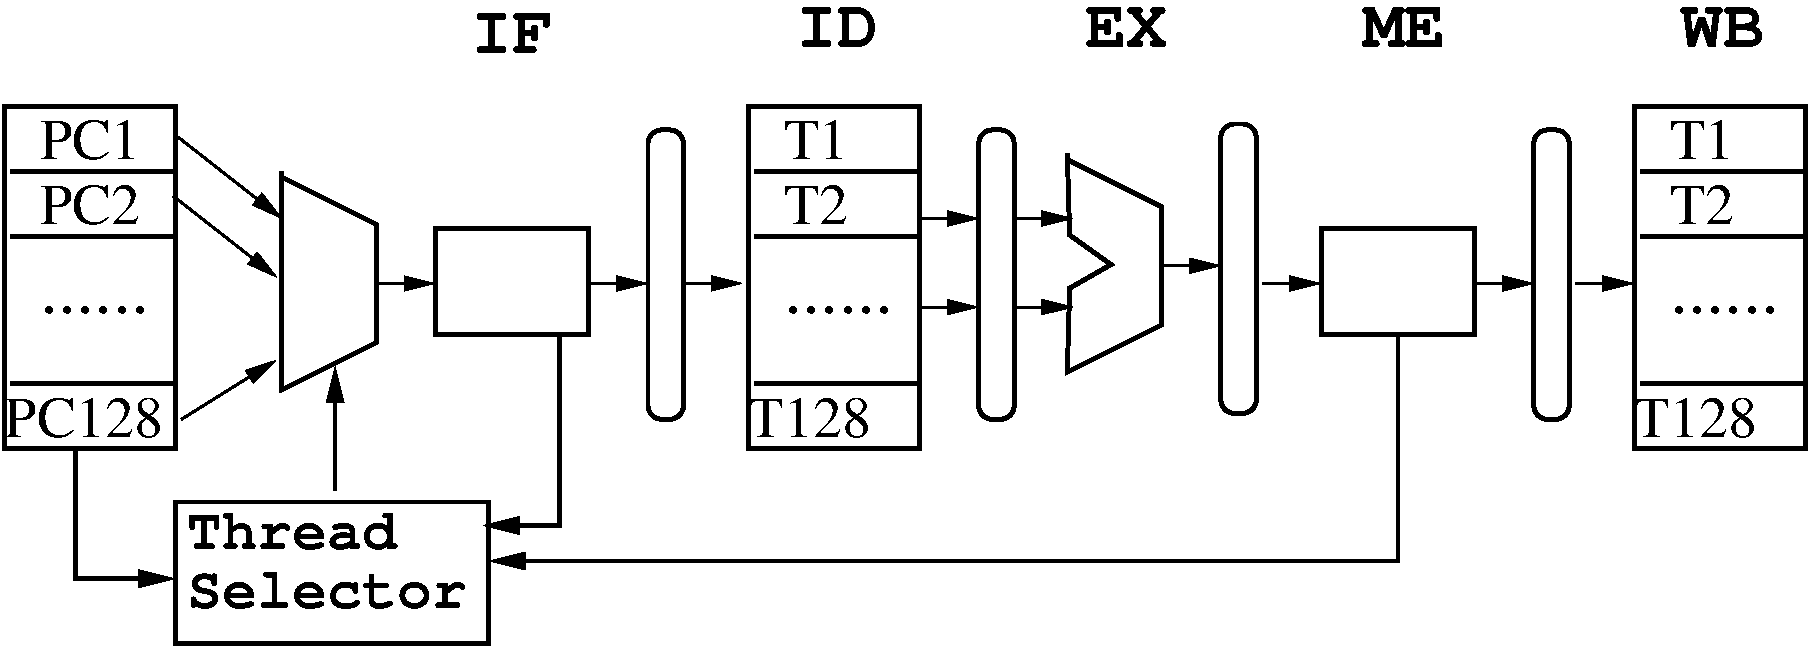
\includegraphics[width=59ex]{Figures/Barrel}
\column{0.31\textwidth}
Figure shows a 5-stage pipeline which 128 {\sc htc}s, which can
        hide long mem-access latencies using no or very large 
        and slow caches without ever starving the pipeline.
\end{columns}

\pause

\begin{itemize}
\item Data/Control/Structural Hazards cannot occur \& Precise Exceptions are
        respected because of the \alert{assumption}.  \alert{Problems are}:
    \begin{itemize}\pause
    \begin{scriptsize}
        \item[1] with current technology 1000s of threads would be needed
                 in workload and such hardware replication would be prohibitive,
        \item[2] memory wall gets larger and larger, \emph{[3]} too different from legacy code
        \item[4] if num running threads $<$ 5 $\Rightarrow$ NOOPs inserted $\Rightarrow$
                    slow sequential execution.\smallskip
    \end  {scriptsize}
    \end{itemize}
\pause
\item CDC 6600 (Control Data Corporation) in \alert{1960s}: 32-way multi-threading (MT).
\item Later in 1980s, Deneclor's HEP: 16-way MT, 8-stage pipeline,  no cache.
\item Denclor's TERA contains 256 Horizon Processors, each a 128-way MT, 3-stage pipeline. 
        PC \& register file replicated.
        No data cache $\Rightarrow$ no cache coherence.\\\emp{Estimated that the pipeline
        is fully utilized even if instrs takes 80 cycles to execute!}
\end{itemize} 
\end{scriptsize}

\end{frame}


\subsection{Interleaved Core Multi-Threading}

\begin{frame}[fragile,t]
\frametitle{Interleaved Core Multi-Threading}
\vspace{-1ex}
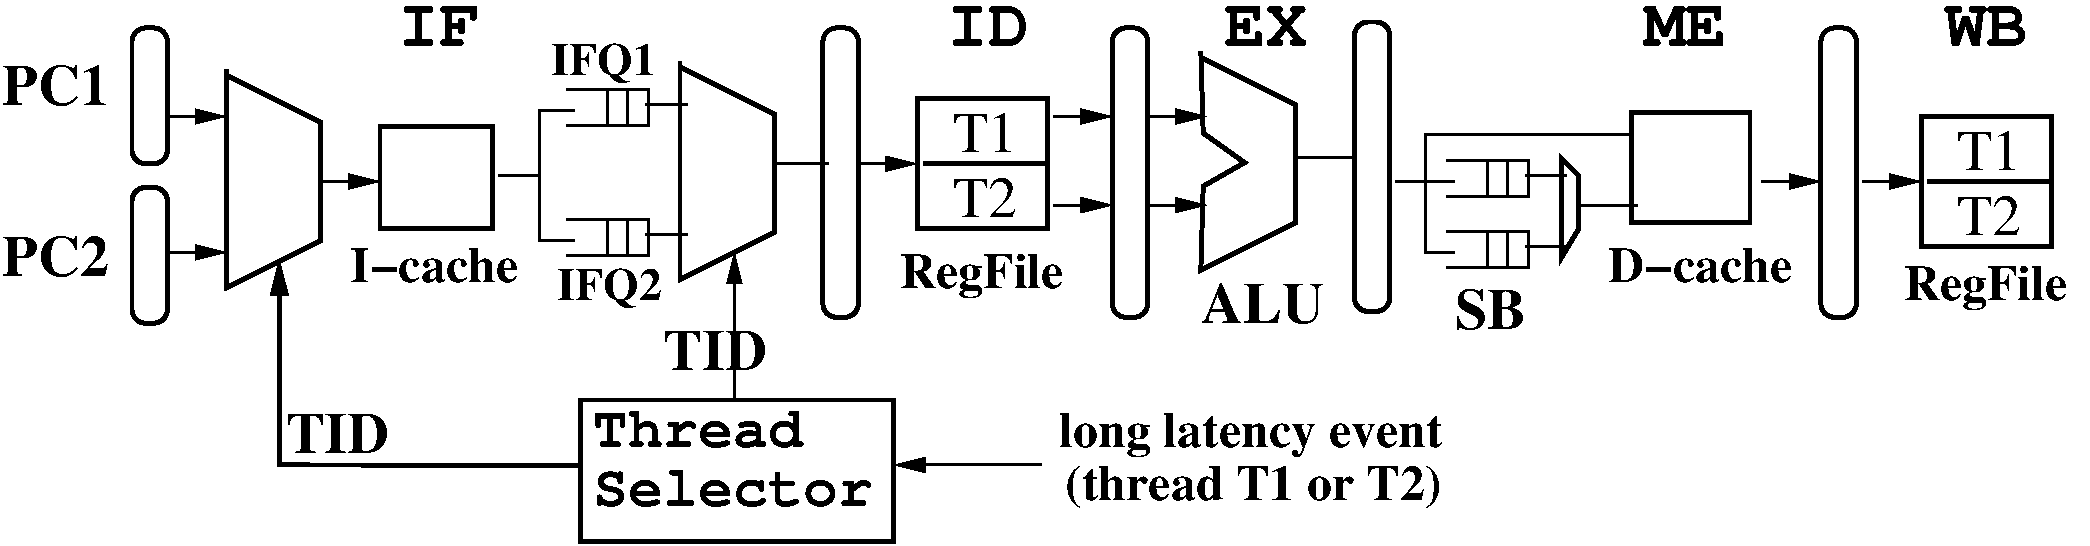
\includegraphics[width=55ex]{Figures/InterleavedMT}
\smallskip

\begin{scriptsize}
\begin{columns}
\column{0.48\textwidth}
Several threads run simultaneously.
Processor fetches, decodes, and schedules 
instrs from $\neq$ threads in consec cycles.\smallskip

A 2-way MT \emp{must have 2 PCs, 2 sets of regs and interrupt flags, 
2 page table base regs}, \emph{BUT shares L1/2 caches \&
pipeline}.\smallskip

Other resources might be replicated, e.g., branch prediction hwd and TLB,
to avoid prediction interferences between tasks.\smallskip

Each instr carries extra bits that identifies its thread id $\Rightarrow$
thread-aware data forwd, stage flushing (exception \& branches).
e.g., on a L1 data-cache miss of {\tt T1}, ME raises a low-level
hwd exception that directs the flushing and insertion
in IFQ1 of the instrs of T1 in ID, EX and ME.\smallskip

\column{0.48\textwidth}
\emp{Seq exec same speed as 5-stage pipeline.}
\emph{Multiple running thds $\Rightarrow$ reduced latencies:}\newline
[1] 5 running thds eliminate all hazards.\newline 
[2] 2 running thds eliminate the bubble of load followed by dependent instr.\smallskip

\alert{SunSparc T1\&T2} (shown in Figure) targets workloads with lots of thds, 
but with little to no FP operations, in which the runtime is dominated by cache misses. 
Decoupling the IF stage via 2 IF-queues smooths out instr delivery in the case of cache 
misses.   Branches are statically predicted by instr bit set by compiler. 
SunSparc T1 has 8 cores, 4-way MT, and SunSparc T2 has 8 cores, 8-way MT each. 

\end{columns}
\end{scriptsize}

\end{frame}


\end{document}
